%%%%%%%%%%%%%%%%%%%%%%%%%%%%%%%%%%%%%%%%%%%%%%%%%%%%%%%%%%%%%%%
%% OXFORD THESIS TEMPLATE

% Use this template to produce a standard thesis that meets the Oxford University requirements for DPhil submission
%
% Originally by Keith A. Gillow (gillow@maths.ox.ac.uk), 1997
% Modified by Sam Evans (sam@samuelevansresearch.org), 2007
% Modified by John McManigle (john@oxfordechoes.com), 2015
% Modified by Ulrik Lyngs (ulrik.lyngs@cs.ox.ac.uk), 2018-, for use with R Markdown
%
% Ulrik Lyngs, 25 Nov 2018: Following John McManigle, broad permissions are granted to use, modify, and distribute this software
% as specified in the MIT License included in this distribution's LICENSE file.
%
% John commented this file extensively, so read through to see how to use the various options.  Remember that in LaTeX,
% any line starting with a % is NOT executed.

%%%%% PAGE LAYOUT
% The most common choices should be below.  You can also do other things, like replace "a4paper" with "letterpaper", etc.

% 'twoside' formats for two-sided binding (ie left and right pages have mirror margins; blank pages inserted where needed):
%\documentclass[a4paper,twoside]{templates/ociamthesis}
% Specifying nothing formats for one-sided binding (ie left margin > right margin; no extra blank pages):
%\documentclass[a4paper]{ociamthesis}
% 'nobind' formats for PDF output (ie equal margins, no extra blank pages):
%\documentclass[a4paper,nobind]{templates/ociamthesis}

% As you can see from the line below, oxforddown uses the a4paper size, 
% and passes in the binding option from the YAML header in index.Rmd:
\documentclass[a4paper, nobind]{templates/ociamthesis}


%%%%% ADDING LATEX PACKAGES
% add hyperref package with options from YAML %
\usepackage[pdfpagelabels]{hyperref}
% handle long urls
\usepackage{xurl}
% change the default coloring of links to something sensible
\usepackage{xcolor}

\definecolor{mylinkcolor}{RGB}{0,0,139}
\definecolor{myurlcolor}{RGB}{0,0,139}
\definecolor{mycitecolor}{RGB}{0,33,71}

\hypersetup{
  hidelinks,
  colorlinks,
  linktocpage=true,
  linkcolor=mylinkcolor,
  urlcolor=myurlcolor,
  citecolor=mycitecolor
}


% add float package to allow manual control of figure positioning %
\usepackage{float}

% enable strikethrough
\usepackage[normalem]{ulem}

% use soul package for correction highlighting
\usepackage{color, soulutf8}
\definecolor{correctioncolor}{HTML}{CCCCFF}
\sethlcolor{correctioncolor}
\newcommand{\ctext}[3][RGB]{%
  \begingroup
  \definecolor{hlcolor}{#1}{#2}\sethlcolor{hlcolor}%
  \hl{#3}%
  \endgroup
}
% stop soul from freaking out when it sees citation commands
\soulregister\ref7
\soulregister\cite7
\soulregister\citet7
\soulregister\autocite7
\soulregister\textcite7
\soulregister\pageref7

%%%%% FIXING / ADDING THINGS THAT'S SPECIAL TO R MARKDOWN'S USE OF LATEX TEMPLATES
% pandoc puts lists in 'tightlist' command when no space between bullet points in Rmd file,
% so we add this command to the template
\providecommand{\tightlist}{%
  \setlength{\itemsep}{0pt}\setlength{\parskip}{0pt}}
 
% allow us to include code blocks in shaded environments

% User-included things with header_includes or in_header will appear here
% kableExtra packages will appear here if you use library(kableExtra)
\usepackage{booktabs}
\usepackage{longtable}
\usepackage{array}
\usepackage{multirow}
\usepackage{wrapfig}
\usepackage{float}
\usepackage{colortbl}
\usepackage{pdflscape}
\usepackage{tabu}
\usepackage{threeparttable}
\usepackage{threeparttablex}
\usepackage[normalem]{ulem}
\usepackage{makecell}
\usepackage{xcolor}


%UL set section header spacing
\usepackage{titlesec}
% 
\titlespacing\subsubsection{0pt}{24pt plus 4pt minus 2pt}{0pt plus 2pt minus 2pt}


%UL set whitespace around verbatim environments
\usepackage{etoolbox}
\makeatletter
\preto{\@verbatim}{\topsep=0pt \partopsep=0pt }
\makeatother


%%%%%%% PAGE HEADERS AND FOOTERS %%%%%%%%%
\usepackage{fancyhdr}
\setlength{\headheight}{15pt}
\fancyhf{} % clear the header and footers
\pagestyle{fancy}
\renewcommand{\chaptermark}[1]{\markboth{\thechapter. #1}{\thechapter. #1}}
\renewcommand{\sectionmark}[1]{\markright{\thesection. #1}} 
\renewcommand{\headrulewidth}{0pt}

\fancyhead[LO]{\emph{\leftmark}} 
\fancyhead[RE]{\emph{\rightmark}} 




% UL page number position 
\fancyfoot[C]{\emph{\thepage}} %regular pages
\fancypagestyle{plain}{\fancyhf{}\fancyfoot[C]{\emph{\thepage}}} %chapter pages




%%%%% SELECT YOUR DRAFT OPTIONS
% This adds a "DRAFT" footer to every normal page.  (The first page of each chapter is not a "normal" page.)

% IP feb 2021: option to include line numbers in PDF

% for line wrapping in code blocks
\usepackage{fancyvrb}
\usepackage{fvextra}
\DefineVerbatimEnvironment{Highlighting}{Verbatim}{breaklines=true, breakanywhere=true, commandchars=\\\{\}}

% for quotations -- loaded here rather than in ociamthesis.cls, as it needs to
% be loaded after fvextra, otherwise we get a warning message
\usepackage{csquotes}

% This highlights (in blue) corrections marked with (for words) \mccorrect{blah} or (for whole
% paragraphs) \begin{mccorrection} . . . \end{mccorrection}.  This can be useful for sending a PDF of
% your corrected thesis to your examiners for review.  Turn it off, and the blue disappears.
\correctionstrue


%%%%% BIBLIOGRAPHY SETUP
% Note that your bibliography will require some tweaking depending on your department, preferred format, etc.
% If you've not used LaTeX before, I recommend just using pandoc for citations -- this is what's used unless you specific e.g. "citation_package: natbib" in index.Rmd
% If you're already a LaTeX pro and are used to natbib or something, modify as necessary.

% this allows the latex template to handle pandoc citations
\newlength{\cslhangindent}
\setlength{\cslhangindent}{1.5em}
\newlength{\csllabelwidth}
\setlength{\csllabelwidth}{3em}
\newlength{\cslentryspacingunit} % times entry-spacing
\setlength{\cslentryspacingunit}{\parskip}
\newenvironment{CSLReferences}[2] % #1 hanging-ident, #2 entry spacing
 {% don't indent paragraphs
  \setlength{\parindent}{0pt}
  % turn on hanging indent if param 1 is 1
  \ifodd #1
  \let\oldpar\par
  \def\par{\hangindent=\cslhangindent\oldpar}
  \fi
  % set entry spacing
  \setlength{\parskip}{1mm}
  \setlength{\baselineskip}{6mm}
 }%
 {}
\usepackage{calc}
\newcommand{\CSLBlock}[1]{#1\hfill\break}
\newcommand{\CSLLeftMargin}[1]{\parbox[t]{\csllabelwidth}{#1}}
\newcommand{\CSLRightInline}[1]{\parbox[t]{\linewidth - \csllabelwidth}{#1}\break}
\newcommand{\CSLIndent}[1]{\hspace{\cslhangindent}#1}




% Uncomment this if you want equation numbers per section (2.3.12), instead of per chapter (2.18):
%\numberwithin{equation}{subsection}


%%%%% THESIS / TITLE PAGE INFORMATION
% Everybody needs to complete the following:
\title{Integrative Analysis of Omics\\
Data with Biological Knowledge in\\
Translational Medicine}
\author{Ferran Briansó}
\college{Facultat de Biologia\\
Departament de Genètica, Microbiologia i Estadística}

% Master's candidates who require the alternate title page (with candidate number and word count)
% must also un-comment and complete the following three lines:

% Uncomment the following line if your degree also includes exams (eg most masters):
%\renewcommand{\submittedtext}{Submitted in partial completion of the}
% Your full degree name.  (But remember that DPhils aren't "in" anything.  They're just DPhils.)
\degree{Doctor of Philosophy}

% Term and year of submission, or date if your board requires (eg most masters)
\degreedate{XXXX XX 2024}


%%%%% YOUR OWN PERSONAL MACROS
% This is a good place to dump your own LaTeX macros as they come up.

% To make text superscripts shortcuts
\renewcommand{\th}{\textsuperscript{th}} % ex: I won 4\th place
\newcommand{\nd}{\textsuperscript{nd}}
\renewcommand{\st}{\textsuperscript{st}}
\newcommand{\rd}{\textsuperscript{rd}}

%%%%% THE ACTUAL DOCUMENT STARTS HERE
\begin{document}

%%%%% CHOOSE YOUR LINE SPACING HERE
% This is the official option.  Use it for your submission copy and library copy:
\setlength{\textbaselineskip}{22pt plus2pt}
% This is closer spacing (about 1.5-spaced) that you might prefer for your personal copies:
%\setlength{\textbaselineskip}{18pt plus2pt minus1pt}

% You can set the spacing here for the roman-numbered pages (acknowledgements, table of contents, etc.)
\setlength{\frontmatterbaselineskip}{17pt plus1pt minus1pt}

% UL: You can set the line and paragraph spacing here for the separate abstract page to be handed in to Examination schools
\setlength{\abstractseparatelineskip}{13pt plus1pt minus1pt}
\setlength{\abstractseparateparskip}{0pt plus 1pt}

% UL: You can set the general paragraph spacing here - I've set it to 2pt (was 0) so
% it's less claustrophobic
\setlength{\parskip}{2pt plus 1pt}

%
% Customise title page
%
\def\crest{{\includegraphics[width=8cm]{templates/logo\_UBblanc.png}}}
\renewcommand{\university}{Universitat de Barcelona}
\renewcommand{\submittedtext}{A thesis submitted for the degree of}
\renewcommand{\thesistitlesize}{\fontsize{22pt}{28pt}\selectfont}
\renewcommand{\gapbeforecrest}{25mm}
\renewcommand{\gapaftercrest}{25mm
}


% Leave this line alone; it gets things started for the real document.
\setlength{\baselineskip}{\textbaselineskip}


%%%%% CHOOSE YOUR SECTION NUMBERING DEPTH HERE
% You have two choices.  First, how far down are sections numbered?  (Below that, they're named but
% don't get numbers.)  Second, what level of section appears in the table of contents?  These don't have
% to match: you can have numbered sections that don't show up in the ToC, or unnumbered sections that
% do.  Throughout, 0 = chapter; 1 = section; 2 = subsection; 3 = subsubsection, 4 = paragraph...

% The level that gets a number:
\setcounter{secnumdepth}{2}
% The level that shows up in the ToC:
\setcounter{tocdepth}{1}


%%%%% ABSTRACT SEPARATE
% This is used to create the separate, one-page abstract that you are required to hand into the Exam
% Schools.  You can comment it out to generate a PDF for printing or whatnot.

% JEM: Pages are roman numbered from here, though page numbers are invisible until ToC.  This is in
% keeping with most typesetting conventions.
\begin{romanpages}

% Title page is created here
\maketitle

%%%%% DEDICATION
\begin{dedication}
  For XXXXX XXXXXX
\end{dedication}

%%%%% ACKNOWLEDGEMENTS


\begin{acknowledgements}
 	\ldots{} \ldots{} \ldots{} \ldots{}

 \begin{flushright}
 Ferran Brians\'o \\
 Matar\'o, BCN \\
 XX XXXXXX 2024
 \end{flushright}
\end{acknowledgements}



%%%%% ABSTRACT


\renewcommand{\abstracttitle}{Abstract (wip)}
\begin{abstract}
	Over the past decade, advancements in omics technologies have facilitated the high-throughput monitoring of molecular and organism processes. These techniques have been widely applied to identify biological agents and to characterize biochemical systems, often focusing on the discovery of therapeutic targets and biomarkers related with specific diseases (\protect\hyperlink{ref-cisek_application_2016}{Cisek et al., 2016}),(\protect\hyperlink{ref-wang_proteomics_2014}{K. Wang et al., 2014}),(\protect\hyperlink{ref-wang_circulating_2014}{F. Wang et al., 2014}). While many single-omic approaches target comprehensive analysis of genes (genomics), mRNA (transcriptomics), proteins (proteomics), and metabolites (metabolomics) among other, there is still field to improve omics data analyses through integrative methods (\protect\hyperlink{ref-wanichthanarak_genomic_2015}{Wanichthanarak et al., 2015}),(\protect\hyperlink{ref-gomez-cabrero_data_2014}{Gomez-Cabrero et al., 2014}). In this sense, the integrative point of view defined in the paragraph above, applied to multi-omics data, is a promising approach to achieve better biomarker development in biomedical research projects, and this is the core idea of this work.

As the field of omics has evolved from analyzing a unique type of data to multiple types, it has been natural to extend the previous use of multivariate techniques to this new situation. With this aim classical and new multivariate techniques have been applied to the analysis of multi-omics datasets. Many of these techniques are dimension reduction methods that aim at finding main sources of variability in the data while maximizing some information characteristic such as the variance of each dataset, the correlation between groups of variables or other. Examples of such techniques are well consolidated methods such as Principal Component Analysis (PCA), Singular Value Decomposition (SVD), Correspondence Analysis (CA), and Partial Least Squares (PLS). Besides these more ``novel'' approaches have been used such as: Principal Components Regression, Coinertia and Multiple Coinertia Analysis, Generalized SVD, Sparse PLS, Multiple Factor Analysis (MFA), or combined versions of them (\protect\hyperlink{ref-mwheelock_trials_2013}{M. Wheelock \& E. Wheelock, 2013}),(\protect\hyperlink{ref-le_cao_sparse_2009}{Lê Cao et al., 2009}),(\protect\hyperlink{ref-culhane_cross-platform_2003}{Culhane et al., 2003}). Publications such as (\protect\hyperlink{ref-meng_dimension_2016}{Meng et al., 2016}), (\protect\hyperlink{ref-cavill_transcriptomic_2016}{Cavill et al., 2016}), (\protect\hyperlink{ref-wu_selective_2019}{Wu et al., 2019}), (\protect\hyperlink{ref-subramanian_multi-omics_2020}{Subramanian et al., 2020}), (\protect\hyperlink{ref-krassowski_state_2020}{Krassowski et al., 2020}), and (\protect\hyperlink{ref-cantini_benchmarking_2021}{Cantini et al., 2021}), are good reviews of the state of the art of using multivariate and joint reduction methods for Integrative Multi-Omics Analysis.

Dimension reduction methods, especially those that are able to deal with situations that are typical from the omics context (with many more variables than samples, or possibly sparse matrices with many missing values), have been of great help in visualizing datasets or even for performing variable selection to find biomarkers for a given situation (\protect\hyperlink{ref-wu_selective_2019}{Wu et al., 2019}). There is however one point where they underperform other approaches, that is, the difficulty in interpreting results from a biological point of view. This is relatively reasonable, because the most of these methods work by creating new variables that are some type of linear combination from the original ones. While this is useful, for example, for removing redundancy, this does not provide any clues on what these new dimensions may mean from a biological point of view.

This problem has been known since the beginning of using multivariate methods with omics data, but only a few approaches have been taken to deal with this. The first attempts to introduce biological information in the analyses consisted of using the most well-known database of biological functions, the Gene Ontology (GO) (\protect\hyperlink{ref-ashburner_gene_2000}{Ashburner et al., 2000}). Fellenberg (\protect\hyperlink{ref-busold_integration_2005}{Busold et al., 2005}) introduces a way to integrate Gene Ontology information with Correspondence Analysis to facilitate the interpretation of microarray data. De Tayrac et al. (\protect\hyperlink{ref-de_tayrac_simultaneous_2009}{Tayrac et al., 2009}) applies multiple factor analysis to the integrative analysis of microarray and DNA copy number data. They apply GO Terms on data visualizations by treating these terms as supplemental information. In recent years the representation of biological knowledge has shifted from Gene Ontology to using Gene Sets (\protect\hyperlink{ref-huang_bioinformatics_2009}{Huang et al., 2009}). Meng and Culhane (\protect\hyperlink{ref-meng_dimension_2016}{Meng et al., 2016}) have introduced the Integrative Clustering with Gene Set Analysis where gene set expression analysis is performed based on multiple omics data; and Tyekucheva et al. (\protect\hyperlink{ref-tyekucheva_integrating_2011}{Tyekucheva et al., 2011}), go one step further and use the results of Gene Set Expression Analysis (GSEA) to integrate different omics data.

The previous approaches show several things: Although the idea that integrating quantitative data with biological knowledge may increase interpretability, the number of successful attempts to do this is still small. In this thesis, the use of either classical GO Terms or more flexible annotations (Gene Sets or custom annotations), will be combined with different approaches, and combinations of them if needed, to guide integrative analysis and to improve its biological interpretability from the point of view of the biomedical researchers.
\end{abstract}



%%%%% MINI TABLES
% This lays the groundwork for per-chapter, mini tables of contents.  Comment the following line
% (and remove \minitoc from the chapter files) if you don't want this.  Un-comment either of the
% next two lines if you want a per-chapter list of figures or tables.
\dominitoc % include a mini table of contents

% This aligns the bottom of the text of each page.  It generally makes things look better.
\flushbottom

% This is where the whole-document ToC appears:
\tableofcontents

\listoffigures
	\mtcaddchapter
  	% \mtcaddchapter is needed when adding a non-chapter (but chapter-like) entity to avoid confusing minitoc

% Uncomment to generate a list of tables:
\listoftables
  \mtcaddchapter
%%%%% LIST OF ABBREVIATIONS
% This example includes a list of abbreviations.  Look at text/abbreviations.tex to see how that file is
% formatted.  The template can handle any kind of list though, so this might be a good place for a
% glossary, etc.
% First parameter can be changed eg to "Glossary" or something.
% Second parameter is the max length of bold terms.
\begin{mclistof}{List of Abbreviations}{3.2cm}

\item[1-D, 2-D]

One- or two-dimensional, referring \textbf{in this thesis} to spatial dimensions in an image.

\item[Otter]

One of the finest of water mammals.

\item[Hedgehog]

Quite a nice prickly friend.

\end{mclistof} 


% The Roman pages, like the Roman Empire, must come to its inevitable close.
\end{romanpages}

%%%%% CHAPTERS
% Add or remove any chapters you'd like here, by file name (excluding '.tex'):
\flushbottom

% all your chapters and appendices will appear here
\hypertarget{intro}{%
\chapter{Introduction}\label{intro}}

\chaptermark{Introduction}

\minitoc 

\hypertarget{content-of-the-introductory-text-wip}{%
\section{Content of the introductory text (wip)}\label{content-of-the-introductory-text-wip}}

The general concept of Data Integration can be defined as the combination of data from different sources to provide users with a unified view of the data (\protect\hyperlink{ref-lenzerini_data_2002}{Lenzerini, 2002}). However, the practical meaning of the term Integration may vary from, for instance, the computational combination of data to the combination of studies performed independently, the simultaneous analysis of multiple variables on multiple datasets, or any possible approach for homogeneously querying heterogeneous data sources. Therefore, in many cases, integrative analysis may be preferable to a simple combination of data from distinct sources. Integrative analysis allows not only the combination of heterogeneous data but also the combined use of these data to obtain the most relevant information and, what is better, to be able to extract some information that could not be unveiled by the separate analysis of each of the original data types.

Over the past decade, advancements in omics technologies have facilitated high-throughput monitoring of molecular and organism processes. These techniques have been widely applied to identify biological agents and characterize biochemical systems, often focusing on the discovery of therapeutic targets and biomarkers related to specific diseases (\protect\hyperlink{ref-cisek_application_2016}{Cisek et al., 2016}),(\protect\hyperlink{ref-wang_proteomics_2014}{K. Wang et al., 2014}), and (\protect\hyperlink{ref-wang_circulating_2014}{F. Wang et al., 2014}). Although many single-omic approaches target comprehensive analysis of genes (genomics), mRNA (transcriptomics), proteins (proteomics), and metabolites (metabolomics), among others, there is still a need to improve omics data analyses through integrative methods (\protect\hyperlink{ref-wanichthanarak_genomic_2015}{Wanichthanarak et al., 2015}),(\protect\hyperlink{ref-gomez-cabrero_data_2014}{Gomez-Cabrero et al., 2014}). In this sense, the integrative point of view defined in the paragraph above, applied to multi-omics data, is a promising approach to achieving better biomarker development in biomedical research projects, and this is the core idea of this work.

As the field of omics has evolved from analyzing unique types of data to multiple types, it is natural to extend the previous use of multivariate techniques to this new situation. With this aim, classical and new multivariate techniques have been applied for the analysis of multi-omics datasets. Many of these techniques are dimension reduction methods that aim to find the main sources of variability in the data while maximizing some information characteristics, such as the variance of each dataset and the correlation between groups of variables. Examples of such techniques are well-consolidated methods such as Principal Component Analysis (PCA), Singular Value Decomposition (SVD), Correspondence Analysis (CA), and Partial Least Squares (PLS). Besides these more ``novel'' approaches have been used such as: Principal Components Regression, Coinertia and Multiple Coinertia Analysis, Generalized SVD, Sparse PLS, Multiple Factor Analysis (MFA), or combined versions of them (\protect\hyperlink{ref-mwheelock_trials_2013}{M. Wheelock \& E. Wheelock, 2013}),(\protect\hyperlink{ref-le_cao_sparse_2009}{Lê Cao et al., 2009}),(\protect\hyperlink{ref-culhane_cross-platform_2003}{Culhane et al., 2003}). Publications such as (\protect\hyperlink{ref-meng_dimension_2016}{Meng et al., 2016}), (\protect\hyperlink{ref-cavill_transcriptomic_2016}{Cavill et al., 2016}), (\protect\hyperlink{ref-wu_selective_2019}{Wu et al., 2019}), (\protect\hyperlink{ref-subramanian_multi-omics_2020}{Subramanian et al., 2020}), (\protect\hyperlink{ref-krassowski_state_2020}{Krassowski et al., 2020}), and (\protect\hyperlink{ref-cantini_benchmarking_2021}{Cantini et al., 2021}), are good reviews of the state of the art of using multivariate and joint reduction methods for Integrative Multi-Omics Analysis.

Dimension reduction methods, especially those that are able to deal with situations that are typical of the omics context (with many more variables than samples, or possibly sparse matrices with many missing values), have been of great help in visualizing datasets or even in performing variable selection to find biomarkers for a given situation (\protect\hyperlink{ref-wu_selective_2019}{Wu et al., 2019}). However, there is one point where they underperform other approaches: the difficulty in interpreting results from a biological point of view. This is relatively reasonable because most of these methods work by creating new variables that are a type of linear combination from the original ones. While this is useful, for example, for removing redundancy, it does not provide any clues on what these new dimensions may mean from a biological point of view.

This problem has been known since the introduction of multivariate methods with omics data, but only a few approaches have been taken to deal with this problem. The first attempts to introduce biological information in the analyses consisted of using the most well-known database of biological functions, the Gene Ontology (GO) (\protect\hyperlink{ref-ashburner_gene_2000}{Ashburner et al., 2000}). Fellenberg (\protect\hyperlink{ref-busold_integration_2005}{Busold et al., 2005}) introduces a way to integrate Gene Ontology information with Correspondence Analysis to facilitate the interpretation of microarray data. De Tayrac et al. (\protect\hyperlink{ref-de_tayrac_simultaneous_2009}{Tayrac et al., 2009}) applies multiple factor analysis to the integrative analysis of microarray and DNA copy number data. They applied GO Terms on data visualizations by treating these terms as supplemental information. In recent years, the representation of biological knowledge has shifted from Gene Ontology to Gene Sets (\protect\hyperlink{ref-huang_bioinformatics_2009}{Huang et al., 2009}). Meng and Culhane (\protect\hyperlink{ref-meng_dimension_2016}{Meng et al., 2016}) have introduced the Integrative Clustering with Gene Set Analysis where gene set expression analysis is performed based on multiple omics data; and Tyekucheva et al. (\protect\hyperlink{ref-tyekucheva_integrating_2011}{Tyekucheva et al., 2011}), go one step further and use the results of Gene Set Expression Analysis (GSEA) to integrate different omics data.

Altogether, the previous approaches show several things: Although the idea that integrating quantitative data with biological knowledge may increase interpretability, the number of successful attempts to do this is still small. In this thesis, the use of either classical GO Terms or more flexible annotations (Gene Sets or custom annotations) will be combined with different approaches, and combinations of them, if needed, to guide integrative analysis and improve its biological interpretability from the point of view of biomedical researchers.

\hypertarget{backgroundstate-of-the-art-wip}{%
\section{Background/State of the Art (wip)}\label{backgroundstate-of-the-art-wip}}

Falta desenvolupar punts

\hypertarget{omics-data-analyses-wip}{%
\subsection{Omics data analyses (wip)}\label{omics-data-analyses-wip}}

Omics data encompasses comprehensive information about a biological system, encompassing its entirety. The term ``omics'' originates from the Greek word ``oma,'' meaning ``a collection'' or ``a mass.'' Omics data is generated through high-throughput analysis technologies that enable the measurement of gene expression, protein composition, DNA structure, metabolism, and more.

Among the primary omics data types one can highlight the following:

\begin{itemize}
\tightlist
\item
  Genomics: The study of the genome, which comprises the complete set of genes within an organism.
\item
  Transcriptomics: The investigation of gene expression, focusing on the amount of messenger RNA (mRNA) produced from each gene.
\item
  Proteomics: The examination of proteins, the molecules that carry out the majority of biological functions.
\item
  Metabolomics: The study of metabolism, the ensemble of chemical reactions occurring within an organism.
\item
  Epigenomics: The exploration of changes in gene expression that are not attributed to alterations in DNA sequence.
\end{itemize}

Omics data integration stands as a complex endeavor requiring advanced statistical and computational methods. It is employed for a range of biomedical applications, such as identifying novel genes and proteins linked to diseases, developing new drugs, and enhancing diagnostic accuracy.

3 problemes esencials (veure projecte recerca Alex):

\begin{itemize}
\item
  \textbf{Omics data may be partly incomplete}, especially in multiomics studies, where not all types of data are usually available for all individuals.
\item
  \textbf{The results of these analyses are difficult to interpret}. If we agree that the ultimate goal of many analyzes is a better understanding of the underlying biological processes, for example, in a disease study context, it should be possible to establish a clear relationship between the outcome of an analysis and what this means biologically. And this is not always so.
\item
  \textbf{These kind of data analytics are difficult to standardize}, as it is not easy to make complex pipelines of multi-omics analyses, which integrate multiple processes with multiple sources, easy to reproduce or communicate.
\end{itemize}

Més el problema de la p\textgreater\textgreater n (Dimensionallity Reduction Techniques; The p\textgreater\textgreater n situation)

\hypertarget{the-problem-of-having-partly-incomplete-data}{%
\subsection{The problem of having partly incomplete data}\label{the-problem-of-having-partly-incomplete-data}}

Having partly incomplete data is a common challenge in biomedical multi-omics data analyses, where not all omics layers or samples have complete measurements for all variables of interest. This problem, known as missing data, can hinder the integrative analysis and interpretation of multi-omics datasets.

\textbf{Missing Data Types}: Missing data can occur in various forms in multi-omics datasets. For example, some omics layers may have missing values for certain variables (e.g., genes, proteins, metabolites), or specific samples may be missing data for certain omics layers. This can result from technical limitations, experimental design, or inherent biological variability.(\protect\hyperlink{ref-flores_missing_2023}{Flores et al., 2023})

\textbf{Impact on Analysis}: Incomplete data can introduce biases and distort the results of multi-omics analyses. It can affect downstream statistical analyses, clustering, network inference, and machine learning algorithms, leading to inaccurate or unreliable findings. Addressing missing data appropriately is crucial for obtaining valid and meaningful results. Reference:

\textbf{Missing Data Mechanisms}: Understanding the underlying mechanisms of missing data is essential for selecting appropriate imputation methods. Missing data can occur due to different mechanisms, such as missing completely at random (MCAR), missing at random (MAR), or missing not at random (MNAR). These mechanisms influence the choice of imputation techniques and the assumptions made during data analysis.(\protect\hyperlink{ref-little_missing_2002}{Little \& Rubin, 2002})

\textbf{Imputation Methods}: Imputation techniques are employed to estimate missing values in multi-omics datasets. Various imputation methods, including mean imputation, regression imputation, multiple imputation, and machine learning-based approaches, have been proposed to handle missing data in different omics layers. Each method has its assumptions, strengths, and limitations, and the choice of imputation strategy should be carefully considered. Reference: Buuren, S. V., \& Groothuis-Oudshoorn, K. (2011). mice: Multivariate imputation by chained equations in R. Journal of Statistical Software, 45(3), 1-67.

\textbf{Uncertainty and Sensitivity Analysis}: Dealing with missing data introduces uncertainty in the imputed values and subsequent analyses. Sensitivity analyses, such as multiple imputation and bootstrapping, can help assess the robustness of the results to missing data assumptions and imputation methods. Reference: Sterne, J. A., et al.~(2009). Multiple imputation for missing data in epidemiological and clinical research: Potential and pitfalls. BMJ, 338, b2393.

Addressing the issue of incomplete data in multi-omics analyses is crucial to avoid biased or misleading results. By utilizing appropriate imputation methods and understanding the missing data mechanisms, researchers can mitigate the impact of missing data and enhance the accuracy and reliability of their analyses.

\hypertarget{results-interpretation-in-the-context-of-integrative-multi-omics-data-analyses}{%
\subsection{Results interpretation in the context of integrative multi-omics data analyses}\label{results-interpretation-in-the-context-of-integrative-multi-omics-data-analyses}}

Interpretation of results in integrative multi-omics data analyses is a critical challenge due to the complexity and high dimensionality of the data, as well as the need to integrate information from multiple omics layers. Here, I will explain the problem of result interpretation in this context and provide relevant bibliographic references.

\textbf{Data Integration Challenges}: Integrating multi-omics data involves combining information from different molecular layers such as genomics, transcriptomics, proteomics, and metabolomics. Each omics layer provides a unique perspective on biological processes, and integrating these layers can reveal comprehensive insights. However, interpreting the integrated results becomes challenging due to the heterogeneity and scale differences among the omics data. Reference: Wang, X., \& Zhang, B. (2018). Integrating multiple `omics' data for biomarker discovery and clinical assessment. Molecular \& Cellular Proteomics, 17(6), 991-1003.

\textbf{Dimensionality and Complexity}: Multi-omics data analyses often result in high-dimensional datasets with numerous features, making it difficult to interpret the results directly. The challenge lies in identifying the most relevant features or patterns and extracting meaningful biological insights from the vast amount of data. Reference: Nguyen, T. M., et al.~(2019). Integrative analysis of multi-omics data for discovery and functional studies of complex human diseases. Advances in Genetics, 103, 143-175.

\textbf{Contextual Interpretation}: Interpreting multi-omics results requires considering the biological context, such as pathways, networks, and regulatory interactions. Understanding how different omics layers interact and influence each other within biological systems is crucial for accurate interpretation. Reference: Mei, H., et al.~(2017). The road beyond omics: Integration of multi-omics data for the inference of regulatory networks and precision medicine. Computational and Structural Biotechnology Journal, 15, 359-366.

\textbf{Validation and Biological Significance}: Integrative multi-omics analyses often generate numerous associations, correlations, or biomarkers. However, validating and determining the biological significance of these findings is a key challenge. Experimental validation, functional enrichment analysis, and comparison with existing knowledge are essential for confirming the biological relevance of the results. Reference: Sun, H., et al.~(2020). Strategies for interpreting multi-omics studies in schizophrenia and other neuropsychiatric disorders. Journal of Psychiatric Research, 129, 121-133.

\textbf{Visualization and Interactive Tools}: Visualizing and exploring multi-omics data can aid in result interpretation. Interactive visualization tools that integrate different omics layers, provide network views, and enable user-driven exploration can facilitate the interpretation process. Reference: Swatloski, T., \& et al.~(2020). Multi-Omics Data Integration, Interpretation, and Its Application. Genes, 11(10), 1162.

In summary, the problem of result interpretation in integrative multi-omics data analyses stems from the challenges of data integration, high dimensionality, contextual understanding, validation, and visual exploration. Addressing these challenges requires a combination of statistical methods, biological knowledge, and interactive tools to extract meaningful insights from the integrated data.

\hypertarget{approaches-for-the-biological-and-clinical-interpretation}{%
\subsection{Approaches for the biological and clinical interpretation}\label{approaches-for-the-biological-and-clinical-interpretation}}

The biological and clinical interpretation of multi-omics data analysis results is crucial for gaining insights into the underlying molecular mechanisms, identifying biomarkers, and understanding disease processes.

\begin{enumerate}
\def\labelenumi{\arabic{enumi}.}
\item
  \textbf{Pathway and Functional Enrichment Analysis}: Pathway and functional enrichment analysis aim to identify overrepresented biological pathways, gene sets, or functional categories that are significantly associated with the differentially expressed genes or other omics features. These analyses help in understanding the biological processes, molecular functions, and cellular components that are affected in a particular condition or disease. Citation: Khatri, P., et al.~(2012). Ten years of pathway analysis: Current approaches and outstanding challenges. PLoS Computational Biology, 8(2), e1002375.
\item
  \textbf{Network Analysis}: Network analysis involves the construction and analysis of biological networks, such as gene regulatory networks or protein-protein interaction networks, using multi-omics data. Network-based approaches help in identifying key hub genes, modules, or subnetworks that play important roles in disease progression or phenotype. Citation: Barabási, A. L., et al.~(2011). Network medicine: A network-based approach to human disease. Nature Reviews Genetics, 12(1), 56-68.
\item
  \textbf{Machine Learning and Predictive Modeling}: Machine learning algorithms, such as random forests, support vector machines, or deep learning models, can be applied to multi-omics data to develop predictive models for disease diagnosis, prognosis, or treatment response. These models can uncover potential biomarkers or patterns in multi-omics data and provide insights into disease classification and personalized medicine. Citation: Alizadeh, A. A., et al.~(2000). Prediction of survival in diffuse large-B-cell lymphoma based on the expression of six genes. New England Journal of Medicine, 344(14), 1031-1037.
\item
  \textbf{Integration of Multi-Omics Data}: Integrative analysis methods aim to combine and analyze different omics datasets, such as transcriptomics, proteomics, and epigenomics, to identify molecular interactions and relationships across different layers of biological information. These methods enable a more comprehensive understanding of the molecular mechanisms underlying complex diseases or biological processes. Citation: Liu, Y., et al.~(2014). A survey of integrative analysis methods for multi-omics data. Statistical Methods in Medical Research, 27(11), 3061-3077.
\item
  \textbf{Data Visualization}: Data visualization techniques, such as heatmaps, scatter plots, or network visualizations, play a crucial role in the interpretation of multi-omics data analysis results. Visualizations help in identifying patterns, clusters, and relationships between variables, enabling researchers to generate hypotheses and communicate findings effectively. Citation: Gehlenborg, N., et al.~(2010). Visualization of omics data for systems biology. Nature Methods, 7(3), S56-S68.
\end{enumerate}

These methods, among others, contribute to the biological and clinical interpretation of multi-omics data analysis results, providing insights into disease mechanisms, biomarker discovery, and potential therapeutic targets.

\hypertarget{data-processing-and-standarization}{%
\subsection{Data processing and standarization}\label{data-processing-and-standarization}}

Data processing and standardization are critical steps in biomedical multi-omics data analyses to ensure data quality, comparability, and compatibility across different omics layers and studies. In this context, I will explain the problem of data processing and standardization and provide relevant bibliographic references.

\textbf{Data Preprocessing}: Raw multi-omics data often require preprocessing steps to handle technical variations, correct systematic biases, and remove noise. This may involve background correction, normalization, batch effect removal, and quality control measures to ensure data quality and comparability. Reference: Tarazona, S., et al.~(2015). Data quality aware analysis of differential expression in RNA-seq with NOISeq R/Bioc package. Nucleic Acids Research, 43(21), e140.

\textbf{Integration Challenges}: Integrating multi-omics data involves combining information from different omics layers, which may have distinct measurement scales, dynamic ranges, and data distributions. Harmonizing the data across omics layers is necessary to enable meaningful comparisons and integrative analyses. Reference: Meng, C., et al.~(2014). Dimension reduction techniques for the integrative analysis of multi-omics data. Briefings in Bioinformatics, 17(4), 628-641.

\textbf{Missing Data Handling}: In multi-omics datasets, missing data can be present due to technical limitations or experimental designs. Proper handling of missing data, such as imputation or exclusion strategies, is crucial to avoid biases and ensure accurate analyses. Reference: Zhou, Y., et al.~(2021). Missing data imputation in single-cell RNA sequencing and its implications in integrative multi-omics analysis. Briefings in Bioinformatics, 22(5), bbaa212.

\textbf{Standardization and Metadata}: Standardization of data formats, annotation, and metadata is vital for data sharing, reproducibility, and cross-study comparisons. The use of common data standards and ontologies facilitates data integration and harmonization efforts. Reference: Sansone, S. A., et al.~(2012). Toward interoperable bioscience data. Nature Genetics, 44(2), 121-126.

\textbf{Quality Control}: Implementing quality control measures is essential to identify and remove low-quality or unreliable data points. Quality control procedures can include outlier detection, sample exclusion criteria, and identifying technical artifacts or batch effects. Reference: Leek, J. T., et al.~(2010). Tackling the widespread and critical impact of batch effects in high-throughput data. Nature Reviews Genetics, 11(10), 733-739.

Effective data processing and standardization in multi-omics analyses are crucial for accurate and meaningful interpretations. These steps ensure data quality, comparability, and compatibility, enabling integrative analyses and cross-study comparisons.

\hypertarget{tools-for-the-development-of-bioinformatics-pipelines-in-biomedical-multi-omics-data-integration}{%
\subsection{Tools for the development of bioinformatics pipelines in biomedical multi-omics data integration}\label{tools-for-the-development-of-bioinformatics-pipelines-in-biomedical-multi-omics-data-integration}}

PENDENT DE PRIMERES NOTES

\hypertarget{motivation-for-integrative-analysis}{%
\subsection{Motivation for Integrative analysis}\label{motivation-for-integrative-analysis}}

The fable of the blind men and the elephant ( \url{https://en.wikipedia.org/wiki/Blind_men_and_an_elephant}) is a metaphorical story that can be applied to various contexts, including the motivation behind using distinct omics data types in biomedical integrative data analyses. In this fable, several blind men touch different parts of an elephant and form their own interpretations based on the limited information they gather from their individual experiences. See Figure \ref{fig:fig1-1}. In the parable, several blind men touch different parts of an elephant, but each one perceives only a small aspect of the whole animal. As a result, they form vastly different and often conflicting impressions of what an elephant is. Each blind man, based on his limited sense of touch, describes the elephant differently. One might touch the tail and think the elephant is like a rope, while another feeling the leg believes it's like a tree trunk. Yet another touching the ear might think it's like a fan. None of them, however, comprehends the entirety of the elephant. See Figure \ref{fig:fig1-2}.

\begin{figure}

{\centering 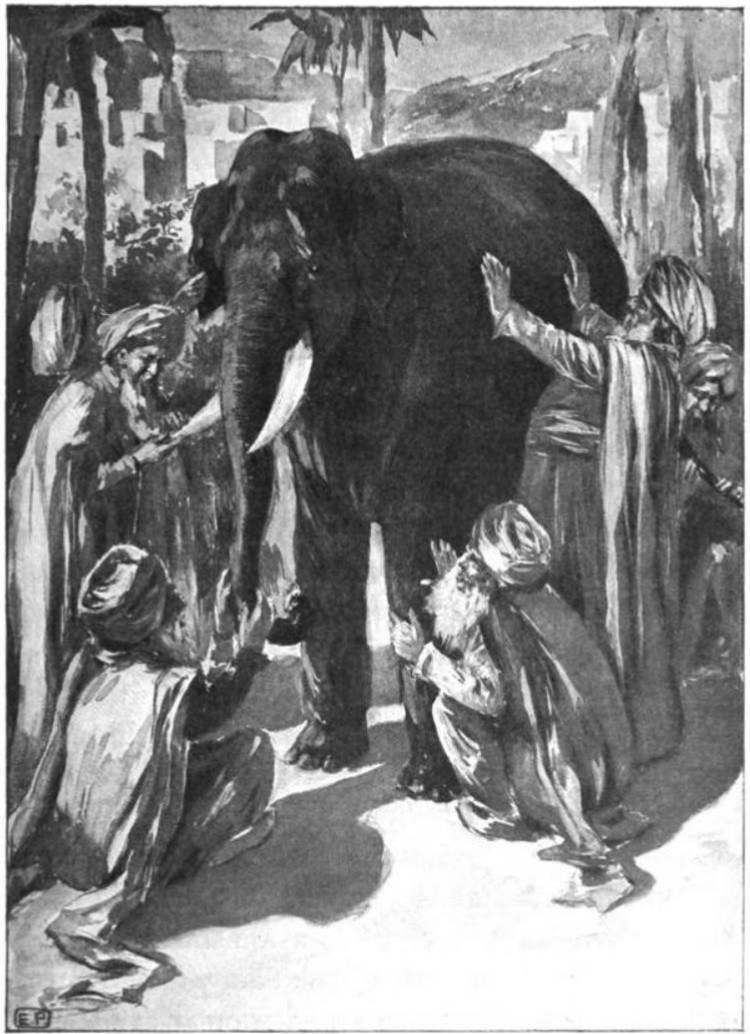
\includegraphics[width=0.95\linewidth]{figures/chapter1/1-1_blind_men} 

}

\caption[The blind men and the elephant]{The blind men and the elephant. By Illustrator unknown - From The Heath readers by grades, D.C. Heath and Company (Boston), p. 69., Public Domain, https://commons.wikimedia.org/w/index.php?curid=4581263}\label{fig:fig1-1}
\end{figure}

The parable is often interpreted to convey the idea that individuals may have partial, subjective truths based on their limited experiences and perspectives. It's a metaphor for the limitations of perception and the importance of considering multiple viewpoints to arrive at a more complete understanding of a complex reality. Similarly, in biomedical research, different omics data types provide distinct perspectives on biological processes, and no single omics layer can fully capture the complexity of the underlying system. Each omics layer, such as genomics, transcriptomics, proteomics, and metabolomics, provides specific insights into different molecular components and interactions. By integrating these diverse data types, we aim to create a more comprehensive and accurate understanding of the biological system, similar to how the blind men can form a more complete understanding of the elephant by sharing and integrating their individual observations.

Each omics data type reveals a specific aspect of biological information. For example, genomics focuses on the DNA sequence, providing insights into genetic variations and potential disease-causing mutations. Transcriptomics examines gene expression levels, helping us understand which genes are active in a given condition. Proteomics investigates the expression and abundance of proteins, shedding light on protein-protein interactions and signaling pathways. Metabolomics analyzes small molecules, providing insights into metabolic pathways and cellular processes.

By integrating these different omics layers, we can overcome the limitations of each individual data type and gain a more holistic understanding of biological phenomena. Integrative multi-omics data analyses enable us to uncover complex relationships, identify key biological pathways, discover biomarkers, and generate more accurate predictions for diseases and therapeutic interventions.

\begin{figure}

{\centering 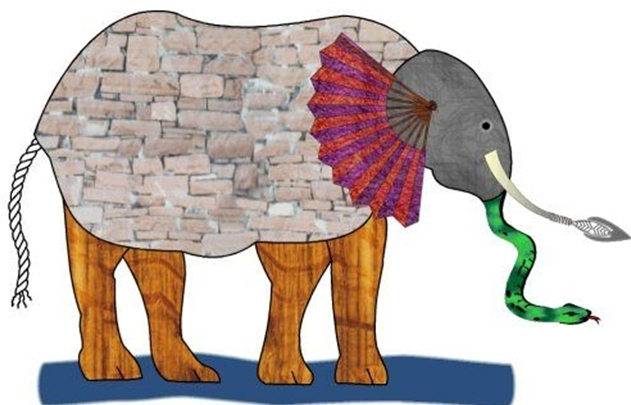
\includegraphics[width=0.95\linewidth]{figures/chapter1/1-2_elephant} 

}

\caption[Reconstruction of the elephant as the blind men perceive it]{Reconstruction of the elephant as the blind men perceive it. Image source: http://doug-johnson.squarespace.com/blue-skunk-blog/2012/12/8/the-blind-men-and-the-elephant.html;jsessionid=30DE43866E1B453471B75CB39688E2CB.v5-web003}\label{fig:fig1-2}
\end{figure}

Just as the blind men needed to collaborate and share their individual perceptions to form a complete understanding of the elephant, biomedical researchers can leverage the strengths of different omics data types and integrate their findings to reveal a more comprehensive picture of biological systems. Integrative approaches allow us to move beyond isolated observations and capture the intricate interplay among genes, proteins, metabolites, and other molecular entities.

In conclusion, the fable of the blind men and the elephant serves as an analogy for the motivation behind using distinct omics data types in biomedical integrative data analyses. Just as the blind men's individual perceptions were limited, focusing on a single omics data type can lead to an incomplete understanding of complex biological processes. Integration of diverse omics data types enables us to overcome these limitations and gain a more comprehensive understanding of the intricacies of living systems.

\textbf{Interpretability is a weak point of most multi omics approaches}

La reducció ve més motivada per la necessitat de destacar els aspectes més rellevants i de que aquests siguin més fàcilment interpretables

\textbf{Methods focus much more on feature selection discovery and interaction highlighting measurement than on clinical or biological interpretability.}

\hypertarget{existing-approaches-for-multi-omics-data-integration}{%
\subsection{Existing approaches for multi-omics data integration}\label{existing-approaches-for-multi-omics-data-integration}}

Maneres de reduir dimensió amb finalitat integració òmiques

MCIA, RGCCA, MFA\ldots{}
\ldots{}(\protect\hyperlink{ref-culhane_cross-platform_2003}{Culhane et al., 2003})
\ldots{}(\protect\hyperlink{ref-cavill_transcriptomic_2016}{Cavill et al., 2016})
\ldots{}(\protect\hyperlink{ref-vahabi_unsupervised_2022}{Vahabi \& Michailidis, 2022})
\ldots{}(\protect\hyperlink{ref-wekesa_review_2023}{Wekesa \& Kimwele, 2023})
\ldots{}(\protect\hyperlink{ref-athieniti_guide_2023}{Athieniti \& Spyrou, 2023})

\hypertarget{revisiuxf3-de-metodes-de-creacio-pipelines}{%
\subsection{Revisió de metodes de creacio pipelines}\label{revisiuxf3-de-metodes-de-creacio-pipelines}}

PENDENT INCLOURE PRIMERES NOTES

\hypertarget{objectives}{%
\chapter{Objectives}\label{objectives}}

\chaptermark{Objectives}

\noindent The main objectives of this work are the following:

\begin{enumerate}
\def\labelenumi{\arabic{enumi}.}
\item
  To make an empirical comparison of some of the currently available dimension reduction techniques applied for the integration of omics data, focused on their ability to include biological annotations,
\item
  To develop methods and workflows able to apply these techniques, focusing on the matching of distinct omics datasets relying on biological knowledge,
\item
  To apply these methods to specific translational biomedical research cases, such as an integrative analysis of transcriptomics and proteomics data to study ischemic stroke, as well as to public datasets, which can be easily shared and are not as restricted by sample sizes as other projects.
\item
  To implement the knowledge acquired with this work into the appropriate bioinformatics tools, e.g.~R packages or web-based tools, that will be used in future biomedical research projects for providing a better interpretation of this kind of studies.
\end{enumerate}

\begin{small}All these objectives are in agreement with the tasks defined within a project partially supported by Grant MTM2015-64465-C2-1-R (MINECO/FEDER) from the Ministerio de Economía y Competitividad (Spain), to which the PhD Thesis proposed here is related.\end{small}

\hypertarget{working-phases-modificar-titols}{%
\section{Working phases (modificar titols)}\label{working-phases-modificar-titols}}

Working phases, with the corresponding steps, followed in order to achieve the above objectives:

\begin{enumerate}
\def\labelenumi{\arabic{enumi}.}
\item
  Application of integrative multi-omics methods to (I) the analysis of specific data sets provided by research units from our former affiliation center, VHIR, and other research institutions that we collaborate with (\protect\hyperlink{ref-rodriguez-hernandez_cinacalcet_2016}{Rodríguez-Hernández et al., 2016}), (\protect\hyperlink{ref-rodriguez-fernandez_phosphatidyl_2018}{Rodriguez-Fernandez et al., 2018}), (\protect\hyperlink{ref-simats_mouse_2020}{Simats et al., 2020}) and (II) to the integrative analysis of larger data sets from public data bases, such as Breast Cancer samples from the TCGA project {[}TCGA Research Network: \url{http://cancergenome.nih.gov/}{]}, {[}TCGA-BRCA Project: \url{https://portal.gdc.cancer.gov/projects/TCGA-BRCA}{]}.
\item
  Development of methods, either in terms of new algorithms or in terms of combinative workflows, which will be able to improve, and facilitate, the analysis and biological interpretation of those data sets to be integrated.
\item
  Implementation of the methods developed for this study in the appropriate bioinformatics tools, such as an R package or a web-based application, to facilitate their use in the context of biomedical research projects.
\end{enumerate}

Here follows a brief description of these main five activities, the methods in which they are initially based, the objectives that they are related to, and the corresponding results:

\begin{enumerate}
\def\labelenumi{\arabic{enumi}.}
\item
  Application of some state-of-the-art methods for integrative multi-omics data analysis to the study of human brain tissue samples, collected by the Neurovascular Diseases Laboratory at Vall d'Hebron Research Institute. This part is already finished, and led to publications in 2018 and 2021 (\protect\hyperlink{ref-simats_mouse_2020}{Simats et al., 2020}), (\protect\hyperlink{ref-ramiro_integrative_2021}{Ramiro et al., 2021}). Researchers obtained different omics data from necropsies, which had been processed to obtain mRNA, microRNA and protein expression values. Each dataset had been first analyzed independently using standard bioinformatics protocols {[}R Development Core Team. 2008{]}. These analyses allowed selecting subsets of relevant features, for each type of data, to be used in the integrative analysis. Among all available options, we decided to use two distinct and complementary approaches: (I) Multiple Co-inertia Analysis implemented in Bioconductor packages made4 (\protect\hyperlink{ref-culhane_made4_2005}{Culhane et al., 2005}) and mogsa (\protect\hyperlink{ref-singh_diablo_2016}{Singh et al., 2016}), and (II) Regularized Canonical Correlation Analysis with Sparse Partial Least Squares regression (sPLS), provided by mixomics R package (\protect\hyperlink{ref-rohart_mixomics_2017}{Rohart et al., 2017}). This work had been presented at some meetings (\protect\hyperlink{ref-brianso_ibc_2016}{Briansó et al., 2016a}), (\protect\hyperlink{ref-brianso_eccb_2016}{Briansó et al., 2016b}), (\protect\hyperlink{ref-garcia-berrocoso_scb_2016}{García-Berrocoso et al., 2016}), (\protect\hyperlink{ref-garcia-berrocoso_scbf_2017}{García-Berrocoso et al., 2017}) and in an already published extended abstract's series book (\protect\hyperlink{ref-brianso_integrative_2017}{Briansó et al., 2017}). This step had been obviously useful for the achievement of the objective number 3 explained in the previous section, which aims on the study of the regulome's response to ischemic stroke, but also useful for detecting the advantages and drawbacks of the methods applied, thus setting the basis for the work regarding to objective number 2.
\item
  Reproduction of the same analyses steps performed in point 1) above with publicly available databases, such as distinct omics data from 150 samples from the TCGA-BRCA collection. This data set contains the expression or abundance of mRNA, miRNA and proteomics for 150 breast cancer samples previously prefiltered, as explained in Rohart et al. (\protect\hyperlink{ref-rohart_mixomics_2017}{Rohart et al., 2017}), and allows identifying a good multi-omics signature to discriminate between Basal, Her2 and Luminal A breast cancer subtypes. This work is already finished, and complies with objectives 3 and 2.
\item
  Use of all the data sets analyzed up to this point to make a comparison of results between the main implemented methods, and eventually some others, which is the aim of objective 1. This is based on quantitative and qualitative comparison and visualization methods, such as those explained by Thallinger (\protect\hyperlink{ref-pucher_comparison_2019}{Pucher et al., 2019}) and Martin (\protect\hyperlink{ref-martin_bisogenet_2010}{Martin et al., 2010}), going from simple Venn diagrams to more complex, network analysis, software such as some specific R packages (\protect\hyperlink{ref-r_core_team_2022}{R Core Team, 2022}) or Cytoscape (\protect\hyperlink{ref-cline_integration_2007}{Cline et al., 2007}). The focus here is to use graphical visualization elements to compare the results of the analyses with and without the addition of biological information.
\item
  Development of new methods and/or workflows in order to improve and/or combine the benefits from the selected approaches, with focus in those allowing the addition of biological significance to the integration process. Here follows an overview of the methods developed to expand the original datasets (X, Y) with annotations (Ax, Ay) to obtain new blocks of data (Nx, Ny,and Nxy). And the workflow has been implemented adapting the integrative pipelines applied so far to the R targets package (\protect\hyperlink{ref-landau_targets_2021}{Landau, 2021}), a pipeline toolkit that improves reproducibility, skipping unnecessary steps already up to date and showing tangible evidence that the results match the underlying code and data. The development of this targets workflow is intended to comply with the objective number 2 of this working plan.
\item
  Implementation of the methods resulting from 4) as a new R package to be submitted to Bioconductor repository (\protect\hyperlink{ref-huber_orchestrating_2015}{Huber et al., 2015}), and, finally, to complete objective 4 of this thesis plan, as a web application (\protect\hyperlink{ref-shiny_2021}{Chang et al., 2021}) to be used in further steps of the current biomedical research projects in which our collaborators are implied, as well as in future studies.
\end{enumerate}

\begin{savequote}
Ein Mann, der recht zu wirken denkt,

Mu\ss\enspace auf das beste Werkzeug halten

\emph{The man who seeks to be approved,}

\emph{must stick to the best tools for it}
\qauthor{--- Goethe's \emph{Faust. Eine Tragödie} (1808).}\end{savequote}



\hypertarget{methods}{%
\chapter{Methodology}\label{methods}}

\chaptermark{Methodology}

\minitoc 

In the context of multi-omics data integration, our proposal relies on the idea that incorporating biological annotations into datasets before integrative analysis enriches outcomes and enhances their biological interpretability. Therefore, augmenting quantitative omics data with contextual biological knowledge will deepen our understanding of complex biological phenomena. To do so, we begin with meticulous data quality assessment and standardization, laying the foundation for reliable analyses. We then infuse biological knowledge using standard biological annotations, creating ``Expanded Datasets'' that provide context for comprehensive analysis. Advanced dimension-reduction techniques can be applied to illuminate hidden patterns and relationships between data sources or blocks, and the semi-automation capabilities of the Targets R package allow us to build an easy-to-use implementation of the process.

\hypertarget{qa}{%
\section{Data Quality Assessment and Format Review}\label{qa}}

Before initiating the integrative analysis, a meticulous evaluation of data quality and format compatibility was conducted to ensure the reliability of the input datasets. This crucial step aimed to identify and rectify discrepancies, inconsistencies, or errors that could potentially impact subsequent analyses. During this process, datasets spanning various omics technologies, including transcriptomics and proteomics, are selectively acquired from reputable sources and repositories. Emphasis was placed on meticulous source selection to guarantee consistency and adherence to standardized formats. Subsequently, the raw omics data underwent a comprehensive preprocessing phase, addressing issues such as missing values, outliers, and normalization. This preprocessing step was indispensable for enhancing data quality and enabling comparability across diverse datasets. Additionally, a thorough review of data formats encompassing file types, column naming conventions, and units of measurement was conducted. Non-standardized data were systematically transformed into a uniform format to streamline the downstream integration processes. Through these procedures, a robust foundation was established for subsequent integrative omics analysis, ensuring coherence and validity of the synthesized biomedical insights.

\bigskip

FALTA DETALLAR AQUI COM SHAN VALIDAT ELS DATASETS DE TCGA (ELS DE STROKE ANIRAN A BANDA)
Explicar aquí els requeriments de format dels data sets d'entrada

Mostrar Figure \ref{fig:fig3-10} i Figure \ref{fig:fig3-9} PERO AQUESTES MILLOR COM A TAULES INTEGRADES a markdown

\begin{figure}

{\centering 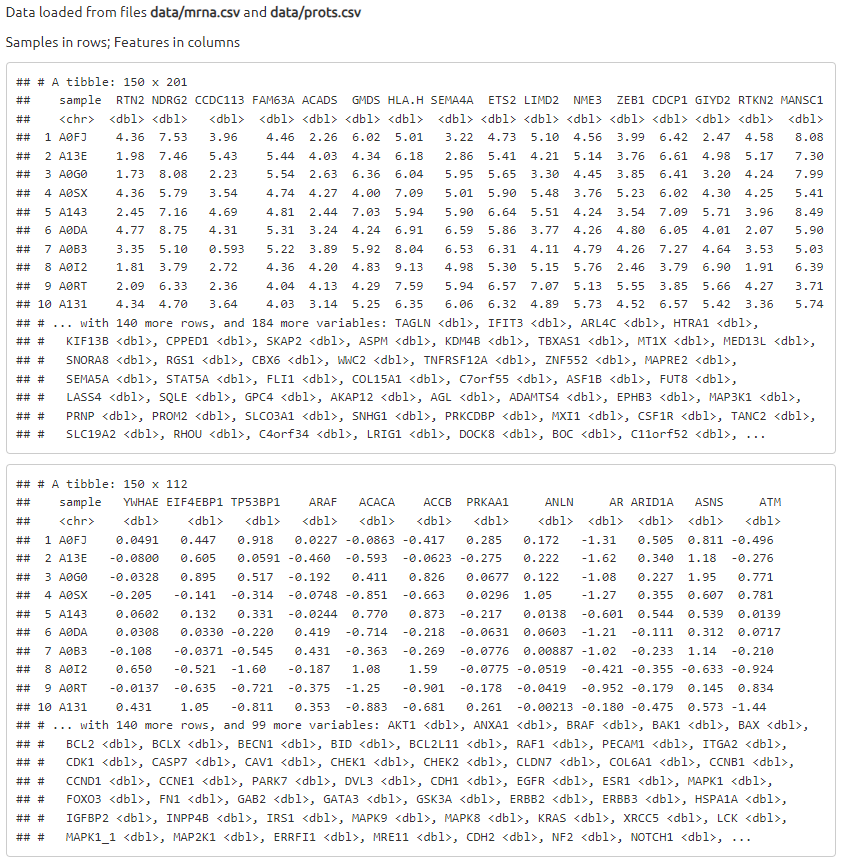
\includegraphics[width=0.95\linewidth]{figures/chapter3/3-10_input_data_R_example} 

}

\caption[Example of gene and protein data loaded in R]{Example of gene expression and protein quantification data as loaded in R}\label{fig:fig3-10}
\end{figure}

\begin{figure}

{\centering 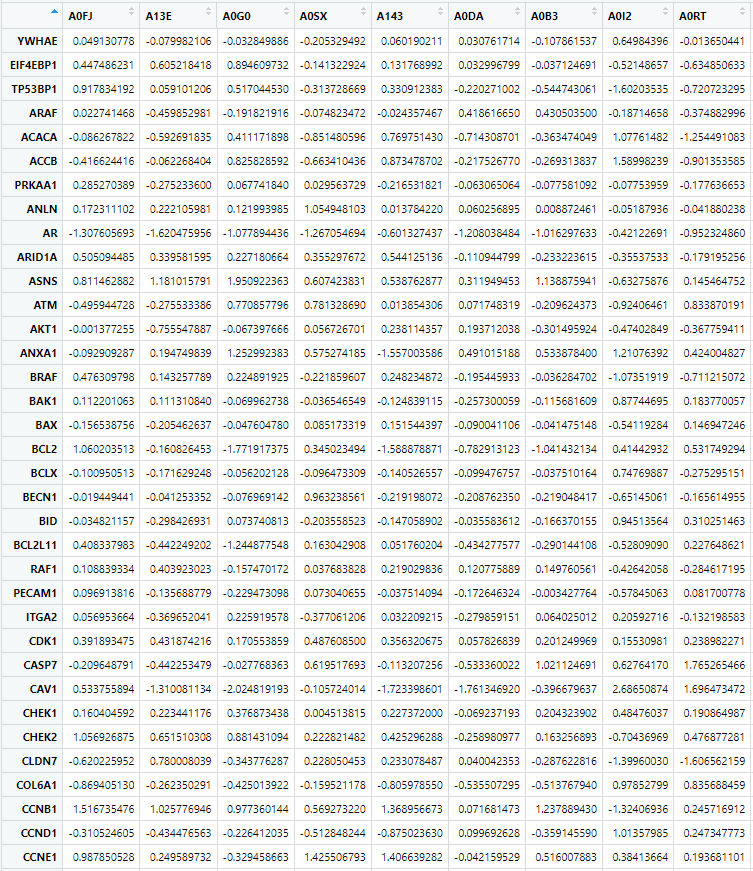
\includegraphics[width=0.95\linewidth]{figures/chapter3/3-9_protein_data_example} 

}

\caption{Example of proteomics input data}\label{fig:fig3-9}
\end{figure}

\clearpage

\hypertarget{preprocess}{%
\section{Preprocessing for Integration of Biological Knowledge: Generating the ``Expanded Datasets''}\label{preprocess}}

The integration of biological knowledge into omics datasets can be achieved through a preprocessing step aimed at expanding the original data matrices with annotations accessed from specialized R libraries, which provided direct access to curated biological databases such as Gene Ontology (GO(\protect\hyperlink{ref-ashburner_gene_2000}{Ashburner et al., 2000})) and biochemical pathways information (e.g., KEGG(\protect\hyperlink{ref-kanehisa_kegg_2000}{Kanehisa \& Goto, 2000})). This process, that combines the annotation of the most significant biological entities with the quantification and integration of their annotation values to the data matrices, ends up with what we term ``Expanded Data Sets'', which include the original biological features (e.g., gene expression or protein quantification values) as well as new variables coming from the annotation of biological terms. The following steps explain this preprocessing procedure in more detail:

\begin{itemize}
\item
  Selected biological annotations: Specialized R libraries, dedicated to biological knowledge integration, are employed to access and retrieve up-to-date annotations from databases such as GO and KEGG.
\item
  Data-Annotation Mapping: Each omics dataset are mapped to the retrieved biological annotations based on identifiers (e.g., gene or protein names) using the capabilities of the R libraries. This step facilitates the linking of omics data to biological knowledge.
\item
  Annotation Integration: The annotated information is integrated, implementing new R functions, into the starting omics datasets, resulting in expanded data matrices that combined the original quantitative omics measurements with new quantified features associated with the given biological annotations.
\end{itemize}

\hypertarget{biosources}{%
\subsection{Selecció de les fonts d'anotacions biològiques}\label{biosources}}

PENDENT DE DETALLAR com escullo les fonts de les anotacions per defecte.
Apuntar que es poden facilitar ja anotacions disponibles prèviament, sempre que compleixin amb el format que s'explica al següent apartat.
Aquestes poden ser estàndard o bé personalitzades a mida de l'usuari (tot i que si es aixi hi ha certes funcionalitats posteriors que no es podran aprofitar).

\clearpage

\hypertarget{bioannotation}{%
\subsection{Anotació de la info biològica}\label{bioannotation}}

COM VAM PLANTEJAR fer l'anotació biologica. Quines opcions i amb quins metodes estadístics/bioinformatics\ldots{}
DUBTO SI LO QUE SEGUEIX NO ANIRIA A RESULTATS

For each input data set, if annotations are not already provided, two distinct basic annotation methods can be performed:

\begin{enumerate}
\def\labelenumi{(\roman{enumi})}
\item
  a basic GO mapping, returning annotations to those GO entities for which we find more than a certain number of features (gene ids coming from our data set, see Figure \ref{fig:fig3-8} for an example) annotated to them,
\item
  a Gene Enrichment Analysis (based on Hypergeometric tests against all GO categories, with FDR correction) is performed in order to retrieve the most relevant annotations to that set of genes/features.(\protect\hyperlink{ref-yu_clusterprofiler_2012}{Yu et al., 2012})
\end{enumerate}

{[}mostrar exemple de llista de gens{]}

\begin{figure}

{\centering 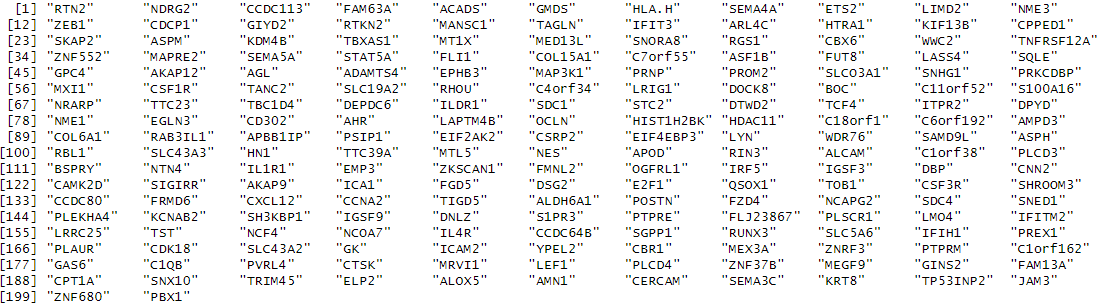
\includegraphics[width=0.95\linewidth]{figures/chapter3/3-8_gene_list} 

}

\caption{List of gene symbols used as example}\label{fig:fig3-8}
\end{figure}

{[}punt de millora, que l'anotacio basica pugui ser tb a KEGG{]}

{[}mostrar formula{]}

es mostra exemple en Figure \ref{fig:fig3-11} POSSIBLE INTEGRAT EN MARKDOWN?

\begin{figure}

{\centering 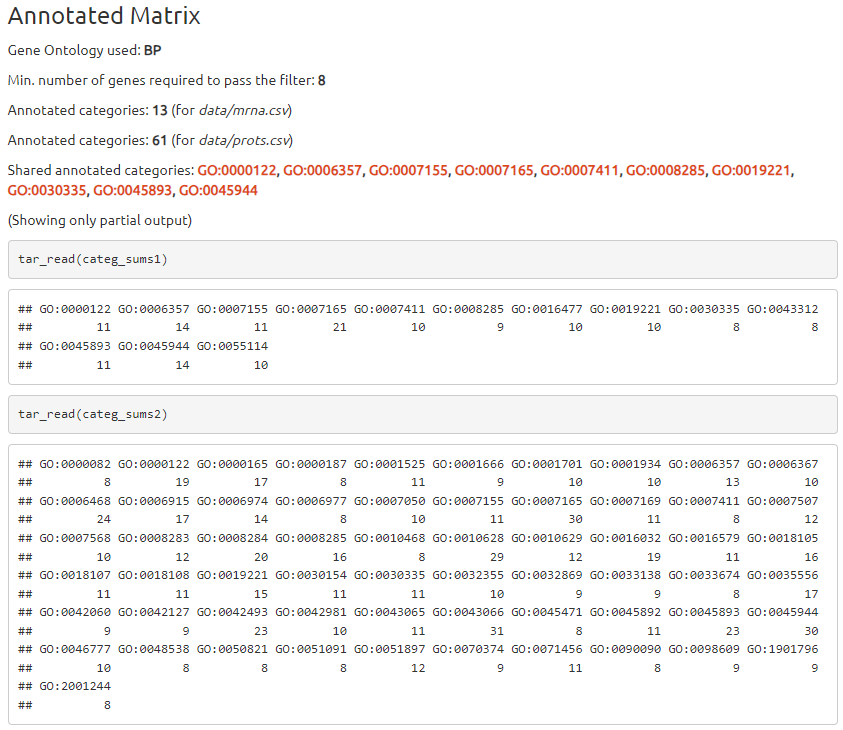
\includegraphics[width=0.95\linewidth]{figures/chapter3/3-11_basicGO_example} 

}

\caption[Example of basic GO annotation by raw count]{Example of basic Go annotation by raw count against GO Biological Processes, setting 8 as minimum number of genes included in the BP entity. Annotation performed separately for gene expression and protein quantification input files}\label{fig:fig3-11}
\end{figure}

{[}comentar aquí l'opció d'afegir les anotacions com a individus suplementaris enlloc de variables Figure \ref{fig:fig3-1} is an example.{]}

\begin{figure}

{\centering 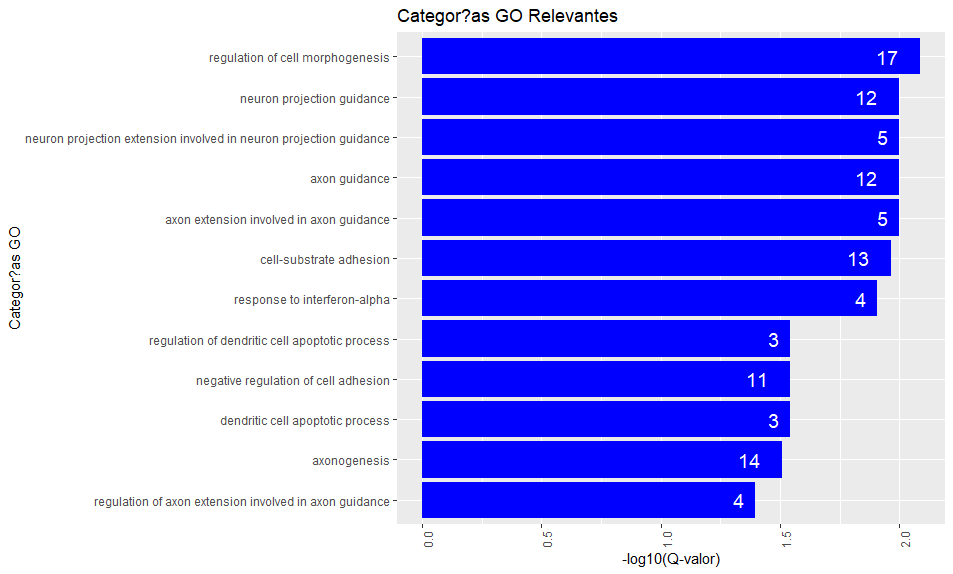
\includegraphics[width=0.95\linewidth]{figures/chapter3/3-12_clusterprofiler_results} 

}

\caption[Example of results from GO annotation]{Example of results from GO annotation. Results of the biological significance analysis performed with the lists of genes against GO through clusterProfiler}\label{fig:fig3-12}
\end{figure}

\clearpage

\begin{figure}

{\centering 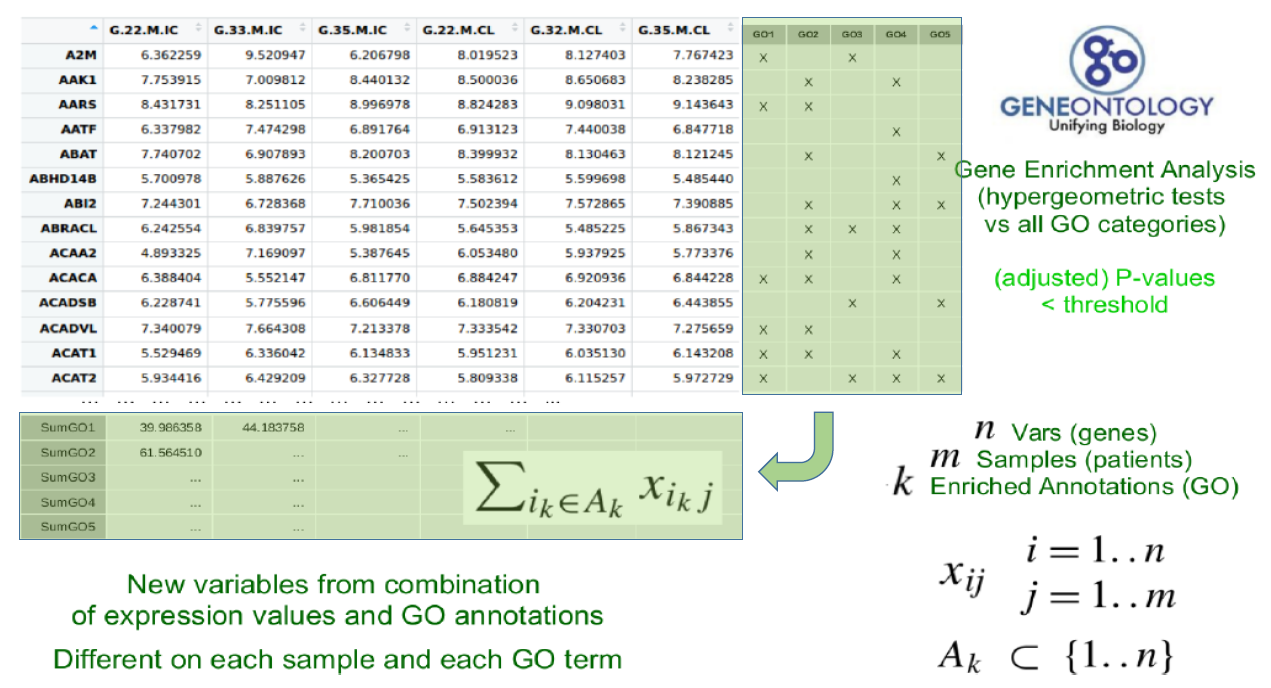
\includegraphics[width=0.95\linewidth]{figures/chapter3/3-1_addition_of_GO_terms} 

}

\caption{Addition of GO terms}\label{fig:fig3-1}
\end{figure}

Alternatively, manual annotations can be provided (eg. GO terms, canonical pathways, or even annotation to custom entities) as an optional input file.

{[}mostrar el format requerit{]}.

Other annotation methods can be implemented, as functions to be used by the main pipeline, if more complex methods for biological information addition are required.

{[}Mostrar el format final de les anotacions, com a matrius dels data sets amb anotacions binàries 1/0 com a columnes extra{]}

EXPANSIO DE LES MATRIUS (numeritzar anotacions, creació de noves vars a partir de les anotacions)

The process starts already having a couple of data sets from distinct 'omics sources {[}punt de millora: admetre 3 o + inputs, comentar més tard a Discussion{]}, mapped to gene ids (in the default case, where GO annotation have been performed), containing the results from a selection of differentially expressed genes or most relevant proteins analysis, or similar.

\clearpage

\hypertarget{biointegration}{%
\subsection{Annotation Integration}\label{biointegration}}

Once the annotations are already computed, mapping each feature of the input data set to the corresponding biological entity, they can be used to generate new features (as new rows), computing the average value {[}punt de millora: funció de ponderació{]} of the expression/intensity values from all original features being mapped to the annotated biological entities.

\begin{figure}

{\centering 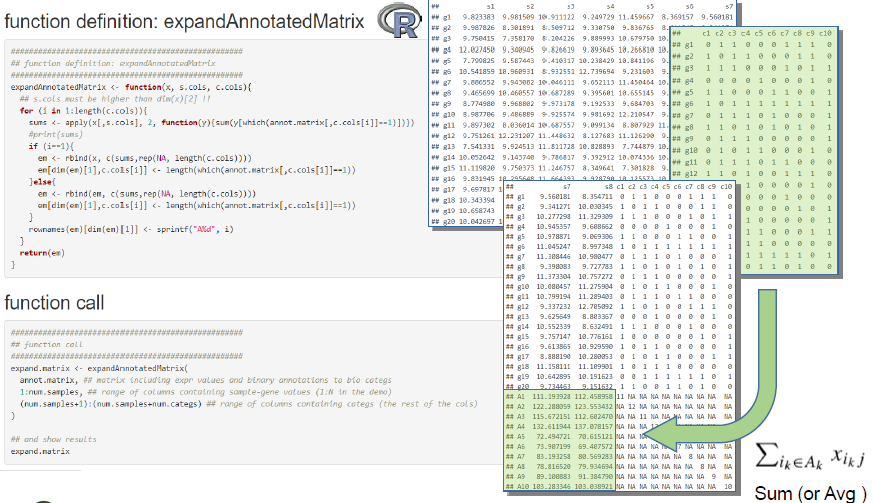
\includegraphics[width=0.95\linewidth]{figures/chapter3/3-2_addition_of_new_feats} 

}

\caption{Addition of news feats}\label{fig:fig3-2}
\end{figure}

\begin{figure}

{\centering 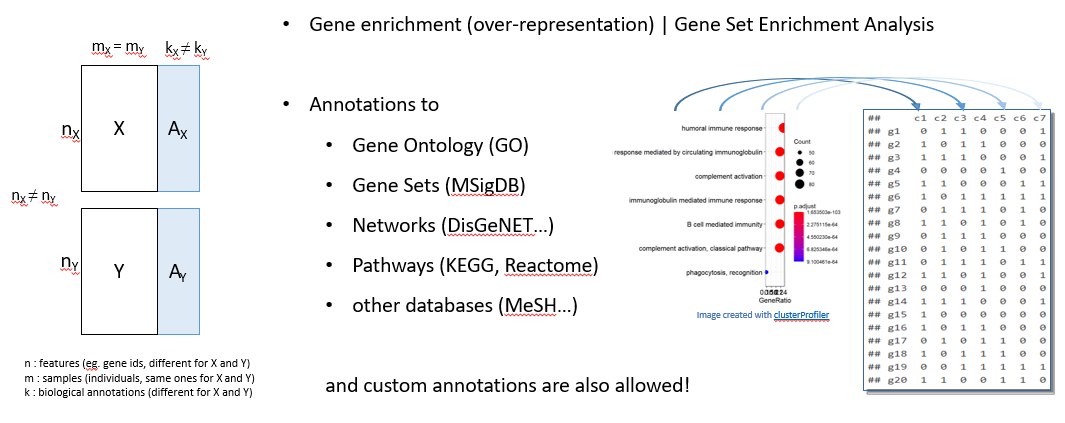
\includegraphics[width=0.95\linewidth]{figures/chapter3/3-3_gene_enrichment_diagram} 

}

\caption{Gene enrichment diagram}\label{fig:fig3-3}
\end{figure}

\begin{figure}

{\centering 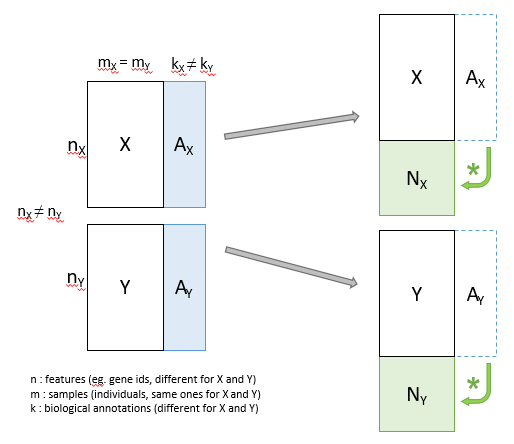
\includegraphics[width=0.95\linewidth]{figures/chapter3/3-4_matrix_expansion_diagram} 

}

\caption{Matrix expansion diagram}\label{fig:fig3-4}
\end{figure}

Once we have the annotated matrices (Figure \ref{fig:fig3-4}, highlighted in blue) we proceed to generate the Expanded matrices (in green) by casting these annotations as numerical values, that is, calculating the average of the numerical expressions of each individual for the variables annotated to each category. This is done with the matrix product of the initial numerical values (expression, proteins\ldots) with the transposed matrices of their annotations, and then with the inverse matrix of a diagonal matrix of the count of how many annotations each category or entity annotated has had.

\begin{figure}

{\centering 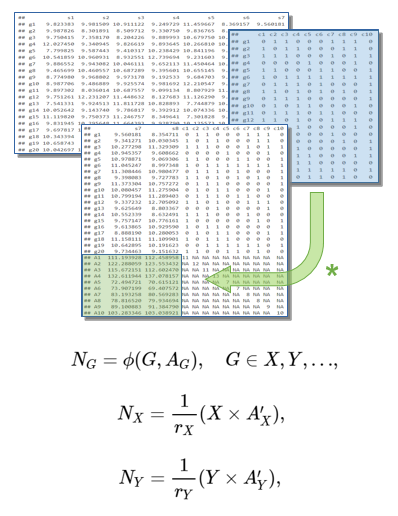
\includegraphics[width=0.95\linewidth]{figures/chapter3/3-5_addition_of_new_feats_2} 

}

\caption{Addition of new feats (2)}\label{fig:fig3-5}
\end{figure}

\begin{figure}

{\centering 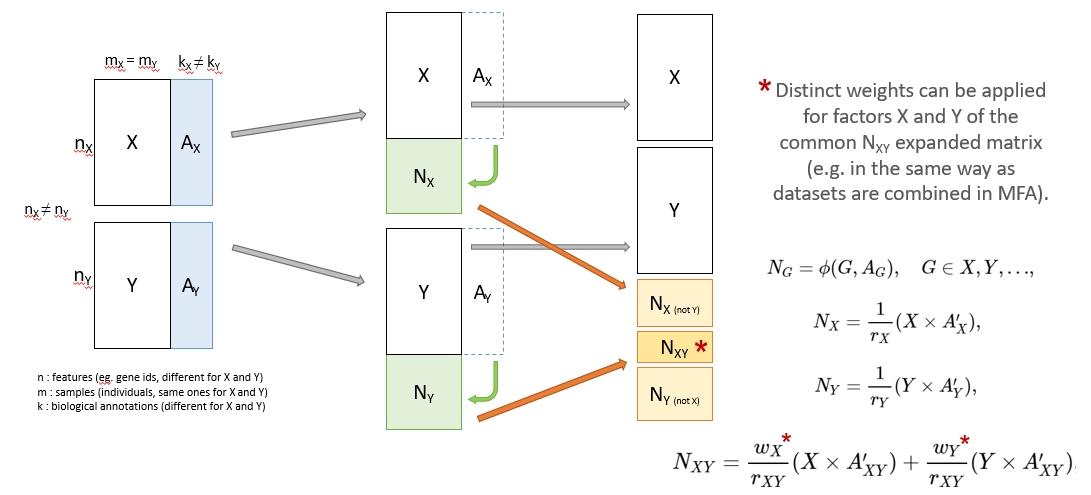
\includegraphics[width=0.95\linewidth]{figures/chapter3/3-6_matrix_expansion_diagram_2} 

}

\caption{Matrix expansion diagram (2)}\label{fig:fig3-6}
\end{figure}

\hypertarget{integrative-analysis-with-joint-dimension-reduction-techniques}{%
\section{Integrative Analysis with Joint Dimension Reduction Techniques}\label{integrative-analysis-with-joint-dimension-reduction-techniques}}

To uncover meaningful insights from the expanded data sets and extract relevant information from the integrated omics and biological knowledge, contrasted joint dimension reduction techniques were employed. These techniques enable the simultaneous analysis of multiple data types and facilitate the identification of key patterns and relationships. The following methods were applied:

\begin{itemize}
\item
  Multiple Factor Analysis (MFA): MFA, adapted for multi-omics data, was utilized to identify sources of variability in the integrated dataset while considering both quantitative omics data and biological annotations. MFA aims to maximize relevant information within the data while accounting for the hierarchical structure of the biological knowledge.
\item
  Multiple Co-Inertia Analysis (MCIA): MCIA, a technique that aligns the covariance structures of multiple datasets, was employed to explore relationships between omics measurements and biological annotations. MCIA seeks to identify common patterns and associations between these data sources.
\item
  Regularized Generalized Canonical Correlation Analysis (RGCCA): RGCCA was used to identify latent variables that capture joint information from omics data and biological annotations. RGCCA extends canonical correlation analysis to handle multi-view data integration and helps reveal correlated features across datasets.
\end{itemize}

PUNTS A INCLOURE:

\begin{itemize}
\item
  Reducció de dimensió. Anàlisi factorial en detall (MFA), + MCIA + RGCCA
\item
  incloure aquí \% variabilitat explicat segons la estructura de la intersecció de les 2 taules (article Lovino 2022)
\item
  avantatge del MFA és que podem definir blocs de variables!
\item
  no mirem unicament si guanyem variabilitat, sino tambe si millorem interpretabilitat biologica
\end{itemize}

\hypertarget{semi-automation-using-the-targets-r-package}{%
\section{Semi-Automation using the Targets R Package}\label{semi-automation-using-the-targets-r-package}}

The semi-automation of the integrative analysis process was facilitated by leveraging the Targets R package, which provides an efficient and user-friendly framework for building and managing complex analysis pipelines. In the development of the Targets pipeline, careful management of functions and parameters was essential to ensure a systematic and reproducible workflow. The following principles were applied:

\begin{itemize}
\item
  Function Modularity: Functions within the Targets pipeline were designed to be modular, focusing on specific tasks or analyses. This modularity enhanced code readability and maintainability.
\item
  Parameterization: Parameters for each function and analysis step were carefully defined, allowing for flexibility and adaptability in the pipeline. This parameterization enabled the adjustment of analysis settings without modifying the underlying code.
\item
  Dependency Management: Dependencies between different analysis steps were explicitly defined within the pipeline. This ensured that each step was executed in the correct order, and dependencies were automatically managed by the Targets package.
\item
  Error Handling: Error handling procedures were implemented to capture and address potential issues during pipeline execution. This included the ability to handle errors, retries, and reporting of errors for troubleshooting. (NO APLICAT ARA PER ARA!)
\end{itemize}

PENDENT A AMPLIAR:

\begin{itemize}
\tightlist
\item
  Introduccio al paquet Targets en general i de les seves caracteristiques\ldots{}
\end{itemize}

The R `targets' package is a powerful tool for building and managing data science and data analysis pipelines. It is primarily designed for workflow automation, dependency management, and parallel processing in R projects. This package is useful for the following purposes:

\begin{enumerate}
\def\labelenumi{\arabic{enumi}.}
\item
  Define and Manage Workflows: You can create a directed acyclic graph (DAG) that represents the workflow of your data analysis or machine learning project. Each node in the graph corresponds to a target, which can be a data file, an R script, or any other computational task.
\item
  Manage Dependencies: `targets' allows you to specify dependencies between targets, ensuring that tasks are executed in the correct order. If a target depends on another target, it won't be executed until its dependencies are up-to-date.
\item
  Parallel Processing: One of the strengths of `targets' is its ability to parallelize tasks. It can automatically determine which targets can be executed concurrently, improving the efficiency of your workflows, especially when working with large datasets or computationally intensive tasks.
\item
  Incremental Builds: When you make changes to your code or data, `targets' can identify the minimal set of targets that need to be recomputed, saving time and computational resources. This is particularly useful for iterative development and experimentation.
\item
  Reports and Logging: `targets' provides tools for generating reports and logging the progress of your workflow, making it easier to track and document your work.
\item
  Integration: It can be seamlessly integrated with other R packages and tools, such as `drake' for more advanced data workflow management.
\end{enumerate}

So, the `targets' package is especially valuable for projects where data processing is a significant component, and you need a structured way to manage the various steps of your analysis or modeling pipeline. It helps ensure that your analyses are reproducible, efficient, and well-documented.

\begin{itemize}
\tightlist
\item
  Sistema que hem aplicat per crear el pipeline amb Targets\ldots{}
\end{itemize}

\begin{figure}

{\centering 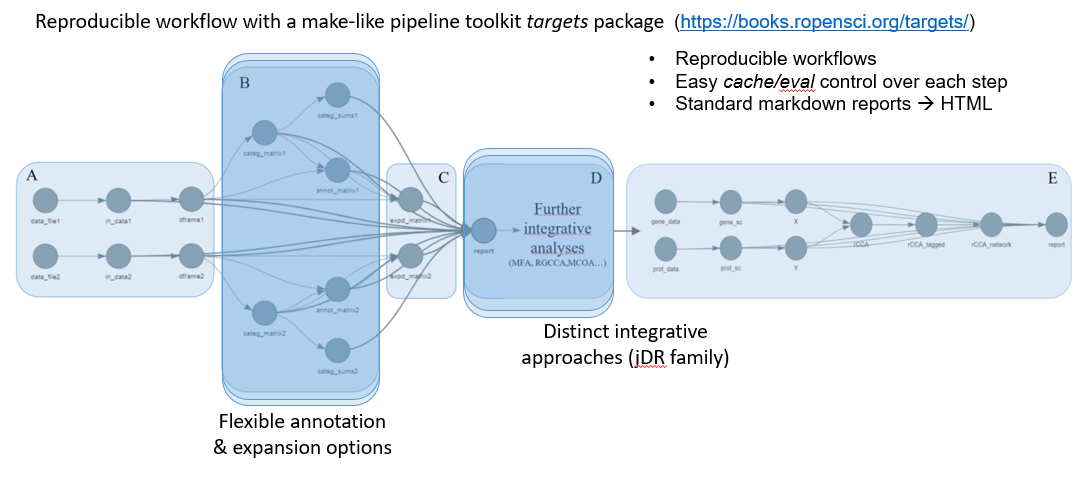
\includegraphics[width=0.95\linewidth]{figures/chapter3/3-7_workflow_overview} 

}

\caption{Workflow overview}\label{fig:fig3-7}
\end{figure}

Targets workflow diagram (Figure \ref{fig:fig3-7}) showing the steps corresponding with the complete process: The pipeline starts from (A) a couple of 'omics-derived input data sets (e.g.~pre-processed gene expression and protein abundance matrices). These are converted to R data frames with features in rows and samples in columns. Then, a data frame containing related annotations (B) is created, or loaded, for each given input matrix, and used to expand these original data, in order to end up with a pair of data frames (C) containing the original values plus the average expression/abundance values of the features related to each annotation as new features in additional rows. After that, distinct Dimension Reduction Methods are applied to perform the integrative analysis (D), and finally, an R markdown report (E) is rendered to show steps and main results of the full process.

\hypertarget{results}{%
\chapter{Results}\label{results}}

\chaptermark{Results}

\minitoc 

Text de presentacio dels resultats\ldots{}

Fer que 4.1 sigui l'actual 4.2 (tota la info d'aplicar el mètode)

ESTRUCTURA DELS RESULTATS:

4.1 Implementació dels algos i les funcions en R

4.2 Pipeline d'anàlisi en amb el paquet `targets'

4.3 Exemples i aplicacions
4.3.1 Results from the analysis of human brain tissue samples
4.3.2 Results from the expansion of omics data with biological annotations
4.3.3 Results from the analysis of 150 TCGA-BRCA samples
4.3.4 Results from the application of MFA on TCGA-BRCA data with, and without, expanded data
4.3.5 \ldots{}

\hypertarget{results-from-the-analysis-of-human-brain-tissue-samples}{%
\section{Results from the analysis of human brain tissue samples}\label{results-from-the-analysis-of-human-brain-tissue-samples}}

\hypertarget{results-from-the-expansion-of-omics-data-with-biological-annotations}{%
\section{Results from the expansion of omics data with biological annotations}\label{results-from-the-expansion-of-omics-data-with-biological-annotations}}

Figure \ref{fig:fig4-1} is an snapshot (F) of one of the heat maps created to show the expanded matrices obtained in (Figures \ref{fig:fig3-4} i \ref{fig:fig3-5} prèvies, de Methods).

\begin{figure}

{\centering 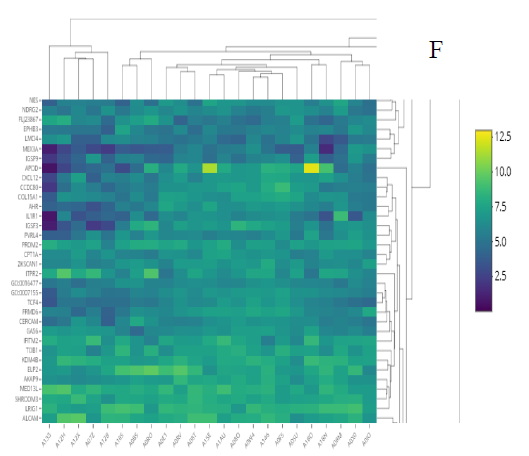
\includegraphics[width=0.95\linewidth]{figures/chapter4/4-1_heatmap_expanded} 

}

\caption{Heapmap of an expanded matrix}\label{fig:fig4-1}
\end{figure}

\hypertarget{results-from-the-analysis-of-150-tcga-brca-samples}{%
\section{Results from the analysis of 150 TCGA-BRCA samples}\label{results-from-the-analysis-of-150-tcga-brca-samples}}

Figure \ref{fig:fig4-2} contains some of the graphical results of the analysis of the 150 samples from TCGA-BRCA: Heat maps (A, C) and association networks (B, D) resulting from the integration by Regularized Canonical Correlations Analysis with mixomics R package. Performed with the original data sets (A, B) or using data expanded with biological annotations to Gene Ontology (C, D), so adding some GO terms to the features from each source, where the outputs contain higher level of information (higher density in both type of plots).

\begin{figure}

{\centering 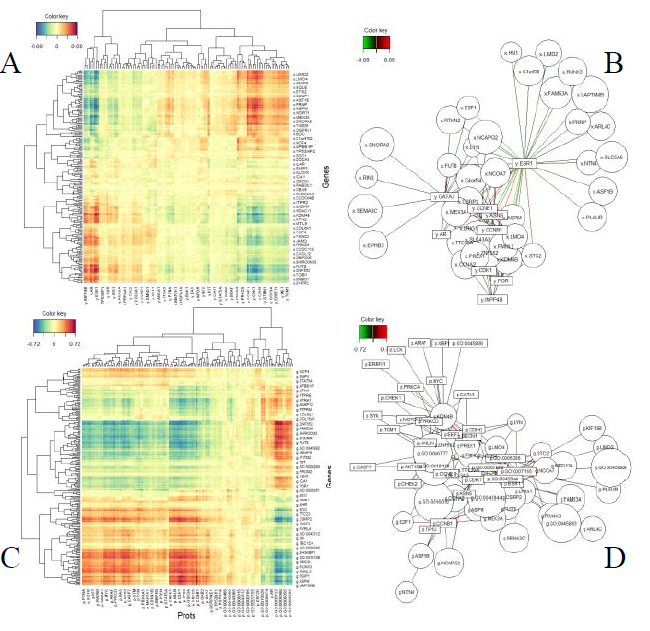
\includegraphics[width=0.95\linewidth]{figures/chapter4/4-2_BRCA_results_overview} 

}

\caption{BRCA results overview}\label{fig:fig4-2}
\end{figure}

\hypertarget{results-from-the-application-of-mfa-on-tcga-brca-data-with-and-without-expanded-data}{%
\section{Results from the application of MFA on TCGA-BRCA data with, and without, expanded data}\label{results-from-the-application-of-mfa-on-tcga-brca-data-with-and-without-expanded-data}}

Figure \ref{fig:fig4-3} includes a Correlation Circle (left), with most relevant genes, proteins and added GO annotations. Distribution of samples (right) along the first two plotted dimensions. Both results coming from the application of Multiple Factor Analysis (FactoMineR and factoextra R packages) performed on the same 150 samples (Basal, Her2 and LuminalA conditions) from TCGA-BRCA.

\begin{figure}

{\centering 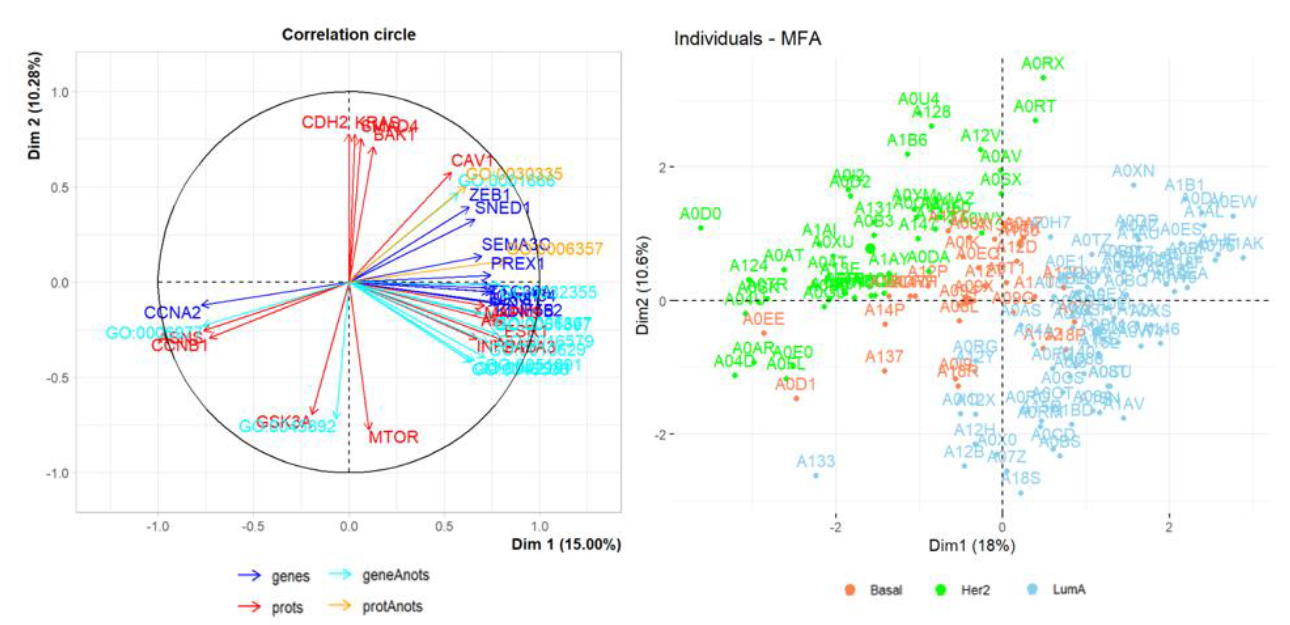
\includegraphics[width=0.95\linewidth]{figures/chapter4/4-3_BRCA_results_withMFA} 

}

\caption{BRCA results with MFA}\label{fig:fig4-3}
\end{figure}

\hypertarget{resultats-de-la-creacio-del-paquet-amb-targets}{%
\section{Resultats de la creacio del paquet amb Targets\ldots{}}\label{resultats-de-la-creacio-del-paquet-amb-targets}}

\clearpage

\hypertarget{discussion}{%
\chapter{Discussion}\label{discussion}}

\chaptermark{Discussion}

\minitoc 

Potser no cal posar la TOC aqui?

Resum de l'article. Apuntant a les conclusions. Comentant problemes i limitacions (emprar combinacions lineals de variables per crear-ne de noves).

Principals problemes i limitacions de la nostra proposta:
* Pendent d'apuntar\ldots{}
* \ldots{}

Possibles extensions i punts de millora. Comentar i descriure cadascun d'ells:

\begin{itemize}
\tightlist
\item
  Poder fer servir 3 o més conjunts de dades òmiques
\item
  que l'anotacio basica pugui ser tb a KEGG i no sols a GO
\item
  opció d'afegir les anotacions com a individus suplementaris enlloc de variables
\item
  Poder ponderar els pesos de les anotacions, segons tipus, data set d'origen, etc.
\item
  Permetre treballar amb dades faltants o, fins i tot, blocs de dades faltants.
\item
  Millorar les opcions del paquet: mètodes d'anotació bio, mètodes d'integració, tipus de gràfics resultants\ldots{}
\end{itemize}

\begin{savequote}
There is grandeur in this view of life, with its several powers, having
been originally breathed into a few forms or into one; and that, whilst
this planet has gone cycling on according to the fixed law of gravity,
from so simple a beginning endless forms most beautiful and most
wonderful have been, and are being, evolved.
\qauthor{--- Darwin's \emph{On the Origin of Species} (1859).}\end{savequote}



\hypertarget{conclusions}{%
\chapter{Conclusions}\label{conclusions}}

\chaptermark{Conclusions}

If we don't want Conclusion to have a chapter number next to it, we can add the \texttt{\{-\}} attribute.

\hypertarget{conclusion-1}{%
\section*{Conclusion 1}\label{conclusion-1}}
\addcontentsline{toc}{section}{Conclusion 1}

The need for a better biological interpretation of multi-omics integrative methods let us to consider the inclusion of biological information during (not after) the analysis process

\hypertarget{conclusion-2}{%
\section*{Conclusion 2}\label{conclusion-2}}
\addcontentsline{toc}{section}{Conclusion 2}

We propose a method focused on the expansion of the starting omics datasets, by adding new annotation-derived features to those matrices, before applying the integrative analysis

\hypertarget{conclusion-3}{%
\section*{Conclusion 3}\label{conclusion-3}}
\addcontentsline{toc}{section}{Conclusion 3}

This approach allows the inclusion of relevant information from the main biological annotation tools, as well as any custom annotation, combined with the use our preferred Dimension Reduction techniques

\hypertarget{conclusion-4}{%
\section*{Conclusion 4}\label{conclusion-4}}
\addcontentsline{toc}{section}{Conclusion 4}

We have implemented a pipeline for reproducible and easy-to-use execution, that facilitates the control of each step, the visualization of results and their reporting to PDF/HTML formats.

\startappendices

\hypertarget{the-first-appendix}{%
\chapter{The First Appendix}\label{the-first-appendix}}

This first appendix includes an R chunk that was hidden in the document (using \texttt{echo\ =\ FALSE}) to help with readibility:

\textbf{In 02-rmd-basics-code.Rmd}

\textbf{And here's another one from the same chapter, i.e.~Chapter \ref{code}:}

\hypertarget{the-second-appendix-for-fun}{%
\chapter{The Second Appendix, for Fun}\label{the-second-appendix-for-fun}}

\hypertarget{references}{%
\chapter*{References}\label{references}}
\addcontentsline{toc}{chapter}{References}

\markboth{References}{}

\hypertarget{refs}{}
\begin{CSLReferences}{1}{0}
\leavevmode\vadjust pre{\hypertarget{ref-ashburner_gene_2000}{}}%
Ashburner, M., Ball, C. A., Blake, J. A., Botstein, D., Butler, H., Cherry, J. M., Davis, A. P., Dolinski, K., Dwight, S. S., Eppig, J. T., Harris, M. A., Hill, D. P., Issel-Tarver, L., Kasarskis, A., Lewis, S., Matese, J. C., Richardson, J. E., Ringwald, M., Rubin, G. M., \& Sherlock, G. (2000). Gene {Ontology}: Tool for the unification of biology. \emph{Nature Genetics}, \emph{25}(1), 25--29. \url{https://doi.org/10.1038/75556}

\leavevmode\vadjust pre{\hypertarget{ref-athieniti_guide_2023}{}}%
Athieniti, E., \& Spyrou, G. M. (2023). A guide to multi-omics data collection and integration for translational medicine. \emph{Computational and Structural Biotechnology Journal}, \emph{21}, 134--149. \url{https://doi.org/10.1016/j.csbj.2022.11.050}

\leavevmode\vadjust pre{\hypertarget{ref-brianso_ibc_2016}{}}%
Briansó, F., García-Berrocoso, T., Montaner, J., \& Sánchez-Pla, A. (2016a). Integrative analysis of transcriptomics and proteomics data for the characterization of brain tissue after ischemic stroke. \emph{XXVIIIth International Biometric Conference IBC2016}.

\leavevmode\vadjust pre{\hypertarget{ref-brianso_eccb_2016}{}}%
Briansó, F., García-Berrocoso, T., Montaner, J., \& Sánchez-Pla, A. (2016b). Multivariate methods for the integrative analysis of transcriptomics and proteomic data in a study on ischemic stroke. \emph{The 15th European Conference on Computational Biology ECCB}.

\leavevmode\vadjust pre{\hypertarget{ref-brianso_integrative_2017}{}}%
Briansó, F., García-Berrocoso, T., Montaner, J., \& Sánchez-Pla, A. (2017). Integrative {Analysis} of {Transcriptomics} and {Proteomics} {Data} for the {Characterization} of {Brain} {Tissue} {After} {Ischemic} {Stroke}. In E. A. Ainsbury, M. L. Calle, E. Cardis, J. Einbeck, G. Gómez, \& P. Puig (Eds.), \emph{Extended {Abstracts} {Fall} 2015} (pp. 21--27). Springer International Publishing. \url{https://doi.org/10.1007/978-3-319-55639-0_4}

\leavevmode\vadjust pre{\hypertarget{ref-busold_integration_2005}{}}%
Busold, C. H., Winter, S., Hauser, N., Bauer, A., Dippon, J., Hoheisel, J. D., \& Fellenberg, K. (2005). Integration of {GO} annotations in {Correspondence} {Analysis}: Facilitating the interpretation of microarray data. \emph{Bioinformatics}, \emph{21}(10), 2424--2429. \url{https://doi.org/10.1093/bioinformatics/bti367}

\leavevmode\vadjust pre{\hypertarget{ref-cantini_benchmarking_2021}{}}%
Cantini, L., Zakeri, P., Hernandez, C., Naldi, A., Thieffry, D., Remy, E., \& Baudot, A. (2021). Benchmarking joint multi-omics dimensionality reduction approaches for the study of cancer. \emph{Nature Communications}, \emph{12}(1), 124. \url{https://doi.org/10.1038/s41467-020-20430-7}

\leavevmode\vadjust pre{\hypertarget{ref-cavill_transcriptomic_2016}{}}%
Cavill, R., Jennen, D., Kleinjans, J., \& Briedé, J. J. (2016). Transcriptomic and metabolomic data integration. \emph{Briefings in Bioinformatics}, \emph{17}(5), 891--901. \url{https://doi.org/10.1093/bib/bbv090}

\leavevmode\vadjust pre{\hypertarget{ref-shiny_2021}{}}%
Chang, W., Cheng, J., Allaire, J., Sievert, C., Schloerke, B., Xie, Y., Allen, J., McPherson, J., Dipert, A., \& Borges, B. (2021). \emph{Shiny: Web application framework for r}. \url{https://CRAN.R-project.org/package=shiny}

\leavevmode\vadjust pre{\hypertarget{ref-cisek_application_2016}{}}%
Cisek, K., Krochmal, M., Klein, J., \& Mischak, H. (2016). The application of multi-omics and systems biology to identify therapeutic targets in chronic kidney disease. \emph{Nephrology Dialysis Transplantation}, \emph{31}(12), 2003--2011. \url{https://doi.org/10.1093/ndt/gfv364}

\leavevmode\vadjust pre{\hypertarget{ref-cline_integration_2007}{}}%
Cline, M. S., Smoot, M., Cerami, E., Kuchinsky, A., Landys, N., Workman, C., Christmas, R., Avila-Campilo, I., Creech, M., Gross, B., Hanspers, K., Isserlin, R., Kelley, R., Killcoyne, S., Lotia, S., Maere, S., Morris, J., Ono, K., Pavlovic, V., \ldots{} Bader, G. D. (2007). Integration of biological networks and gene expression data using {Cytoscape}. \emph{Nature Protocols}, \emph{2}(10), 2366--2382. \url{https://doi.org/10.1038/nprot.2007.324}

\leavevmode\vadjust pre{\hypertarget{ref-culhane_cross-platform_2003}{}}%
Culhane, A. C., Perrière, G., \& Higgins, D. G. (2003). Cross-platform comparison and visualisation of gene expression data using co-inertia analysis. \emph{BMC Bioinformatics}, \emph{4}(1), 59. \url{https://doi.org/10.1186/1471-2105-4-59}

\leavevmode\vadjust pre{\hypertarget{ref-culhane_made4_2005}{}}%
Culhane, A. C., Thioulouse, J., Perrière, G., \& Higgins, D. G. (2005). {MADE4}: An {R} package for multivariate analysis of gene expression data. \emph{Bioinformatics}, \emph{21}(11), 2789--2790. \url{https://doi.org/10.1093/bioinformatics/bti394}

\leavevmode\vadjust pre{\hypertarget{ref-flores_missing_2023}{}}%
Flores, J. E., Claborne, D. M., Weller, Z. D., Webb-Robertson, B.-J. M., Waters, K. M., \& Bramer, L. M. (2023). Missing data in multi-omics integration: {Recent} advances through artificial intelligence. \emph{Frontiers in Artificial Intelligence}, \emph{6}, 1098308. \url{https://doi.org/10.3389/frai.2023.1098308}

\leavevmode\vadjust pre{\hypertarget{ref-garcia-berrocoso_scb_2016}{}}%
García-Berrocoso, T., Goicoechea, L., Simats, A., Briansó, F., Gonzalo, R., Martínez-Saez, E., Moliné, T., Sánchez-Pla, A., \& Montaner, J. (2016). Exploring brain gene expression changes following ischemic stroke through microarrays. \emph{X Simposi de Neurobiologia de La Societat Catalana de Biologia}.

\leavevmode\vadjust pre{\hypertarget{ref-garcia-berrocoso_scbf_2017}{}}%
García-Berrocoso, T., Simats, A., Briansó, F., Llombart, V., Hainard, A., Sánchez-Pla, A., Sanchez, J., \& Montaner, J. (2017). Integrative analysis of transcriptomics and proteomics data for the molecular characterization of human brain after ischemic stroke. \emph{28th Symposium on Cerebral Blood Flow, Metabolism and Function}.

\leavevmode\vadjust pre{\hypertarget{ref-gomez-cabrero_data_2014}{}}%
Gomez-Cabrero, D., Abugessaisa, I., Maier, D., Teschendorff, A., Merkenschlager, M., Gisel, A., Ballestar, E., Bongcam-Rudloff, E., Conesa, A., \& Tegnér, J. (2014). Data integration in the era of omics: Current and future challenges. \emph{BMC Systems Biology}, \emph{8}(2), I1. \url{https://doi.org/10.1186/1752-0509-8-S2-I1}

\leavevmode\vadjust pre{\hypertarget{ref-huang_bioinformatics_2009}{}}%
Huang, D. W., Sherman, B. T., \& Lempicki, R. A. (2009). Bioinformatics enrichment tools: Paths toward the comprehensive functional analysis of large gene lists. \emph{Nucleic Acids Research}, \emph{37}(1), 1--13. \url{https://doi.org/10.1093/nar/gkn923}

\leavevmode\vadjust pre{\hypertarget{ref-huber_orchestrating_2015}{}}%
Huber, W., Carey, V. J., Gentleman, R., Anders, S., Carlson, M., Carvalho, B. S., Bravo, H. C., Davis, S., Gatto, L., Girke, T., Gottardo, R., Hahne, F., Hansen, K. D., Irizarry, R. A., Lawrence, M., Love, M. I., MacDonald, J., Obenchain, V., Oleś, A. K., \ldots{} Morgan, M. (2015). Orchestrating high-throughput genomic analysis with {Bioconductor}. \emph{Nature Methods}, \emph{12}(2), 115--121. \url{https://doi.org/10.1038/nmeth.3252}

\leavevmode\vadjust pre{\hypertarget{ref-kanehisa_kegg_2000}{}}%
Kanehisa, M., \& Goto, S. (2000). {KEGG}: {Kyoto} {Encyclopedia} of {Genes} and {Genomes}. \emph{Nucleic Acids Research}, \emph{28}(1), 27--30. \url{https://doi.org/10.1093/nar/28.1.27}

\leavevmode\vadjust pre{\hypertarget{ref-krassowski_state_2020}{}}%
Krassowski, M., Das, V., Sahu, S. K., \& Misra, B. B. (2020). State of the {Field} in {Multi}-{Omics} {Research}: {From} {Computational} {Needs} to {Data} {Mining} and {Sharing}. \emph{Frontiers in Genetics}, \emph{11}. \url{https://www.frontiersin.org/articles/10.3389/fgene.2020.610798}

\leavevmode\vadjust pre{\hypertarget{ref-landau_targets_2021}{}}%
Landau, W. M. (2021). The targets {R} package: A dynamic {Make}-like function-oriented pipeline toolkit for reproducibility and high-performance computing. \emph{Journal of Open Source Software}, \emph{6}(57), 2959. \url{https://doi.org/10.21105/joss.02959}

\leavevmode\vadjust pre{\hypertarget{ref-le_cao_sparse_2009}{}}%
Lê Cao, K.-A., Martin, P. G., Robert-Granié, C., \& Besse, P. (2009). Sparse canonical methods for biological data integration: Application to a cross-platform study. \emph{BMC Bioinformatics}, \emph{10}(1), 34. \url{https://doi.org/10.1186/1471-2105-10-34}

\leavevmode\vadjust pre{\hypertarget{ref-lenzerini_data_2002}{}}%
Lenzerini, M. (2002). Data integration: A theoretical perspective. \emph{Proceedings of the Twenty-First {ACM} {SIGMOD}-{SIGACT}-{SIGART} Symposium on {Principles} of Database Systems}, 233--246. \url{https://doi.org/10.1145/543613.543644}

\leavevmode\vadjust pre{\hypertarget{ref-little_missing_2002}{}}%
Little, R. J. A., \& Rubin, D. B. (2002). Missing {Data} in {Experiments}. In \emph{Statistical {Analysis} with {Missing} {Data}} (pp. 24--40). John Wiley \& Sons, Ltd. \url{https://doi.org/10.1002/9781119013563.ch2}

\leavevmode\vadjust pre{\hypertarget{ref-mwheelock_trials_2013}{}}%
M. Wheelock, Å., \& E. Wheelock, C. (2013). Trials and tribulations of `omics data analysis: Assessing quality of {SIMCA}-based multivariate models using examples from pulmonary medicine. \emph{Molecular BioSystems}, \emph{9}(11), 2589--2596. \url{https://doi.org/10.1039/C3MB70194H}

\leavevmode\vadjust pre{\hypertarget{ref-martin_bisogenet_2010}{}}%
Martin, A., Ochagavia, M. E., Rabasa, L. C., Miranda, J., Fernandez-de-Cossio, J., \& Bringas, R. (2010). {BisoGenet}: A new tool for gene network building, visualization and analysis. \emph{BMC Bioinformatics}, \emph{11}(1), 91. \url{https://doi.org/10.1186/1471-2105-11-91}

\leavevmode\vadjust pre{\hypertarget{ref-meng_dimension_2016}{}}%
Meng, C., Zeleznik, O. A., Thallinger, G. G., Kuster, B., Gholami, A. M., \& Culhane, A. C. (2016). Dimension reduction techniques for the integrative analysis of multi-omics data. \emph{Briefings in Bioinformatics}, \emph{17}(4), 628--641. \url{https://doi.org/10.1093/bib/bbv108}

\leavevmode\vadjust pre{\hypertarget{ref-pucher_comparison_2019}{}}%
Pucher, B. M., Zeleznik, O. A., \& Thallinger, G. G. (2019). Comparison and evaluation of integrative methods for the analysis of multilevel omics data: A study based on simulated and experimental cancer data. \emph{Briefings in Bioinformatics}, \emph{20}(2), 671--681. \url{https://doi.org/10.1093/bib/bby027}

\leavevmode\vadjust pre{\hypertarget{ref-r_core_team_2022}{}}%
R Core Team. (2022). \emph{R: A language and environment for statistical computing}. R Foundation for Statistical Computing. \url{https://www.R-project.org/}

\leavevmode\vadjust pre{\hypertarget{ref-ramiro_integrative_2021}{}}%
Ramiro, L., García-Berrocoso, T., Briansó, F., Goicoechea, L., Simats, A., Llombart, V., Gonzalo, R., Hainard, A., Martínez-Saez, E., Canals, F., Sanchez, J.-C., Sánchez-Pla, A., \& Montaner, J. (2021). Integrative {Multi}-omics {Analysis} to {Characterize} {Human} {Brain} {Ischemia}. \emph{Molecular Neurobiology}, \emph{58}(8), 4107--4121. \url{https://doi.org/10.1007/s12035-021-02401-1}

\leavevmode\vadjust pre{\hypertarget{ref-rodriguez-fernandez_phosphatidyl_2018}{}}%
Rodriguez-Fernandez, S., Pujol-Autonell, I., Brianso, F., Perna-Barrull, D., Cano-Sarabia, M., Garcia-Jimeno, S., Villalba, A., Sanchez, A., Aguilera, E., Vazquez, F., Verdaguer, J., Maspoch, D., \& Vives-Pi, M. (2018). Phosphatidylserine-{Liposomes} {Promote} {Tolerogenic} {Features} on {Dendritic} {Cells} in {Human} {Type} 1 {Diabetes} by {Apoptotic} {Mimicry}. \emph{Frontiers in Immunology}, \emph{9}, 253. \url{https://doi.org/10.3389/fimmu.2018.00253}

\leavevmode\vadjust pre{\hypertarget{ref-rodriguez-hernandez_cinacalcet_2016}{}}%
Rodríguez-Hernández, C. J., Mateo-Lozano, S., García, M., Casalà, C., Briansó, F., Castrejón, N., Rodríguez, E., Suñol, M., Carcaboso, A. M., Lavarino, C., Mora, J., \& Torres, C. de. (2016). Cinacalcet inhibits neuroblastoma tumor growth and upregulates cancer-testis antigens. \emph{Oncotarget}, \emph{7}(13), 16112--16129. \url{https://doi.org/10.18632/oncotarget.7448}

\leavevmode\vadjust pre{\hypertarget{ref-rohart_mixomics_2017}{}}%
Rohart, F., Gautier, B., Singh, A., \& Cao, K.-A. L. (2017). {mixOmics}: {An} {R} package for `omics feature selection and multiple data integration. \emph{PLOS Computational Biology}, \emph{13}(11), e1005752. \url{https://doi.org/10.1371/journal.pcbi.1005752}

\leavevmode\vadjust pre{\hypertarget{ref-simats_mouse_2020}{}}%
Simats, A., Ramiro, L., García-Berrocoso, T., Briansó, F., Gonzalo, R., Martín, L., Sabé, A., Gill, N., Penalba, A., Colomé, N., Sánchez, A., Canals, F., Bustamante, A., Rosell, A., \& Montaner, J. (2020). A {Mouse} {Brain}-based {Multi}-omics {Integrative} {Approach} {Reveals} {Potential} {Blood} {Biomarkers} for {Ischemic} {Stroke}. \emph{Molecular \& Cellular Proteomics: MCP}, \emph{19}(12), 1921--1936. \url{https://doi.org/10.1074/mcp.RA120.002283}

\leavevmode\vadjust pre{\hypertarget{ref-singh_diablo_2016}{}}%
Singh, A., Gautier, B., Shannon, C. P., Vacher, M., Rohart, F., Tebbutt, S. J., \& Cao, K.-A. L. (2016). \emph{{DIABLO} -- an integrative, multi-omics, multivariate method for multi-group classification}. bioRxiv. \url{https://doi.org/10.1101/067611}

\leavevmode\vadjust pre{\hypertarget{ref-subramanian_multi-omics_2020}{}}%
Subramanian, I., Verma, S., Kumar, S., Jere, A., \& Anamika, K. (2020). Multi-omics {Data} {Integration}, {Interpretation}, and {Its} {Application}. \emph{Bioinformatics and Biology Insights}, \emph{14}, 1177932219899051. \url{https://doi.org/10.1177/1177932219899051}

\leavevmode\vadjust pre{\hypertarget{ref-de_tayrac_simultaneous_2009}{}}%
Tayrac, M. de, Lê, S., Aubry, M., Mosser, J., \& Husson, F. (2009). Simultaneous analysis of distinct {Omics} data sets with integration of biological knowledge: {Multiple} {Factor} {Analysis} approach. \emph{BMC Genomics}, \emph{10}(1), 32. \url{https://doi.org/10.1186/1471-2164-10-32}

\leavevmode\vadjust pre{\hypertarget{ref-tyekucheva_integrating_2011}{}}%
Tyekucheva, S., Marchionni, L., Karchin, R., \& Parmigiani, G. (2011). Integrating diverse genomic data using gene sets. \emph{Genome Biology}, \emph{12}(10), R105. \url{https://doi.org/10.1186/gb-2011-12-10-r105}

\leavevmode\vadjust pre{\hypertarget{ref-vahabi_unsupervised_2022}{}}%
Vahabi, N., \& Michailidis, G. (2022). Unsupervised {Multi}-{Omics} {Data} {Integration} {Methods}: {A} {Comprehensive} {Review}. \emph{Frontiers in Genetics}, \emph{13}. \url{https://www.frontiersin.org/articles/10.3389/fgene.2022.854752}

\leavevmode\vadjust pre{\hypertarget{ref-wang_circulating_2014}{}}%
Wang, F., Chen, C., \& Wang, D. (2014). Circulating {microRNAs} in cardiovascular diseases: From biomarkers to therapeutic targets. \emph{Frontiers of Medicine}, \emph{8}(4), 404--418. \url{https://doi.org/10.1007/s11684-014-0379-2}

\leavevmode\vadjust pre{\hypertarget{ref-wang_proteomics_2014}{}}%
Wang, K., Huang, C., \& Nice, E. (2014). Proteomics, genomics and transcriptomics: {Their} emerging roles in the discovery and validation of colorectal cancer biomarkers. \emph{Expert Review of Proteomics}, \emph{11}. \url{https://doi.org/10.1586/14789450.2014.894466}

\leavevmode\vadjust pre{\hypertarget{ref-wanichthanarak_genomic_2015}{}}%
Wanichthanarak, K., Fahrmann, J. F., \& Grapov, D. (2015). Genomic, {Proteomic}, and {Metabolomic} {Data} {Integration} {Strategies}. \emph{Biomarker Insights}, \emph{10}(Suppl 4), 1--6. \url{https://doi.org/10.4137/BMI.S29511}

\leavevmode\vadjust pre{\hypertarget{ref-wekesa_review_2023}{}}%
Wekesa, J. S., \& Kimwele, M. (2023). A review of multi-omics data integration through deep learning approaches for disease diagnosis, prognosis, and treatment. \emph{Frontiers in Genetics}, \emph{14}. \url{https://www.frontiersin.org/articles/10.3389/fgene.2023.1199087}

\leavevmode\vadjust pre{\hypertarget{ref-wu_selective_2019}{}}%
Wu, C., Zhou, F., Ren, J., Li, X., Jiang, Y., \& Ma, S. (2019). A {Selective} {Review} of {Multi}-{Level} {Omics} {Data} {Integration} {Using} {Variable} {Selection}. \emph{High-Throughput}, \emph{8}(1), 4. \url{https://doi.org/10.3390/ht8010004}

\leavevmode\vadjust pre{\hypertarget{ref-yu_clusterprofiler_2012}{}}%
Yu, G., Wang, L.-G., Han, Y., \& He, Q.-Y. (2012). {clusterProfiler}: An {R} {Package} for {Comparing} {Biological} {Themes} {Among} {Gene} {Clusters}. \emph{OMICS : A Journal of Integrative Biology}, \emph{16}(5), 284--287. \url{https://doi.org/10.1089/omi.2011.0118}

\end{CSLReferences}

%%%%% REFERENCES


\end{document}
